\documentclass[twoside,a4paper]{article}

% Some basic packages
\usepackage[utf8]{inputenc}
\usepackage[T1]{fontenc}
\usepackage{textcomp}
\usepackage[french]{babel}
\usepackage{url}
\usepackage{graphicx}
\usepackage{float}
%\usepackage{booktabs}
\usepackage{fontenc}

\usepackage{hyperref}
\hypersetup{
    colorlinks=true,
    linkcolor=blue,
    filecolor=magenta,      
    urlcolor=cyan,
    }

\urlstyle{same}
%\pdfminorversion=7

% Don't indent paragraphs, leave some space between them
\usepackage{parskip}

% Hide page number when page is empty
\usepackage{emptypage}
\usepackage{subcaption}
\usepackage{multicol}
\usepackage{xcolor}

% Other font I sometimes use.
% \usepackage{cmbright}

% Math stuff
\usepackage{amsmath, amsfonts, mathtools, amsthm, amssymb}
% Fancy script capitals
\usepackage{mathrsfs}
\usepackage{cancel}
% Bold math
\usepackage{bm}
% Some shortcuts
\newcommand\N{\ensuremath{\mathbb{N}}}
\newcommand\R{\ensuremath{\mathbb{R}}}
\newcommand\Z{\ensuremath{\mathbb{Z}}}
\renewcommand\O{\ensuremath{\emptyset}}
\newcommand\Q{\ensuremath{\mathbb{Q}}}
\newcommand\C{\ensuremath{\mathbb{C}}}
\newcommand\Qp{ \ensuremath {\mathbb{Q}_p} }
\newcommand\Zp{ \ensuremath{ \mathbb {Z}_p }} 
\newcommand\val{ \ensuremath{\text{val}_p} }  
\renewcommand\P{ \mathcal{P} } 
\newcommand\Pn{ \mathcal{P}_n \left( \Qp \right)} 
% Easily typeset systems of equations (French package)
\usepackage{systeme}

% Put x \to \infty below \lim
\let\svlim\lim\def\lim{\svlim\limits}

%Make implies and impliedby shorter
\let\implies\Rightarrow
\let\impliedby\Leftarrow
\let\iff\Leftrightarrow
\let\epsilon\varepsilon

% Add \contra symbol to denote contradiction
\usepackage{stmaryrd} % for \lightning
\newcommand\contra{\scalebox{1.5}{$\lightning$}}

\let\phi\varphi

% Command for short corrections
% Usage: 1+1=\correct{3}{2}

\definecolor{correct}{HTML}{009900}
\newcommand\correct[2]{\ensuremath{\:}{\color{red}{#1}}\ensuremath{\to }{\color{correct}{#2}}\ensuremath{\:}}
\newcommand\green[1]{{\color{correct}{#1}}}

% horizontal rule
\newcommand\hr{
    \noindent\rule[0.5ex]{\linewidth}{0.5pt}
}

% hide parts
\newcommand\hide[1]{}

% si unitx
\usepackage{siunitx}
\sisetup{locale = FR}

% Environments
\makeatother
% For box around Definition, Theorem, \ldots
\usepackage{mdframed}
\mdfsetup{skipabove=1em,skipbelow=0em}
\theoremstyle{definition}
\newmdtheoremenv[nobreak=true]{définition}{Définition}
\newmdtheoremenv[nobreak=true]{propriete}{Propriété}
\newmdtheoremenv[nobreak=true]{consequence}{Conséquence}
\newmdtheoremenv[nobreak=true]{lemme}{Lemme}
\newmdtheoremenv[nobreak=true]{proposition}{Proposition}
\newmdtheoremenv[nobreak=true]{theoreme}{Théorème}
\newmdtheoremenv[nobreak=true]{loi}{Loi}
\newmdtheoremenv[nobreak=true]{postulat}{Postulat}
\newmdtheoremenv{conclusion}{Conclusion}
\newmdtheoremenv{corollaire}{Corollaire}
\newmdtheoremenv{corrollaire}{Corollaire}
\newmdtheoremenv{conjecture}{Conjecture}
\newtheorem*{rappel}{Rappel}
\newtheorem*{remarque}{Remarque}
\newtheorem*{notation}{Notation}
\newtheorem*{observation}{Observation}
\newtheorem*{exo}{Exercice}
\newtheorem*{praktisch}{Praktisch}
\newtheorem*{probleme}{Problème}
\newtheorem*{terminologie}{Terminologie}
\newtheorem*{application}{Application}
\newtheorem*{uovt}{UOVT}
\newtheorem*{ex}{Exemple}
\newtheorem*{vraag}{Vraag}

\newmdtheoremenv[nobreak=true]{definition}{Definition}
\newtheorem*{eg}{Example}
%\newtheorem*{notation}{Notation}
\newtheorem*{previouslyseen}{As previously seen}
\newtheorem*{remark}{Remark}
\newtheorem*{note}{Note}
\newtheorem*{problem}{Problem}
\newtheorem*{observe}{Observe}
\newtheorem*{property}{Property}
\newtheorem*{intuition}{Intuition}
\newmdtheoremenv[nobreak=true]{prop}{Proposition}
\newmdtheoremenv[nobreak=true]{theorem}{Theorem}
\newmdtheoremenv[nobreak=true]{corollary}{Corollary}

% End example and intermezzo environments with a small diamond (just like proof
% environments end with a small square)
\usepackage{etoolbox}
\AtEndEnvironment{vb}{\null\hfill$\diamond$}%
\AtEndEnvironment{intermezzo}{\null\hfill$\diamond$}%
% \AtEndEnvironment{opmerking}{\null\hfill$\diamond$}%

% Fix some spacing
% http://tex.stackexchange.com/questions/22119/how-can-i-change-the-spacing-before-theorems-with-amsthm
\makeatletter
\def\thm@space@setup{%
  \thm@preskip=\parskip \thm@postskip=0pt
}


% Exercise 
% Usage:
% \oefening{5}
% \suboefening{1}
% \suboefening{2}
% \suboefening{3}
% gives
% Oefening 5
%   Oefening 5.1
%   Oefening 5.2
%   Oefening 5.3
\newcommand{\oefening}[1]{%
    \def\@oefening{#1}%
    \subsection*{Oefening #1}
}

\newcommand{\suboefening}[1]{%
    \subsubsection*{Oefening \@oefening.#1}
}


% \lecture starts a new lecture (les in dutch)
%
% Usage:
% \lecture{1}{di 12 feb 2019 16:00}{Inleiding}
%
% This adds a section heading with the number / title of the lecture and a
% margin paragraph with the date.

% I use \dateparts here to hide the year (2019). This way, I can easily parse
% the date of each lecture unambiguously while still having a human-friendly
% short format printed to the pdf.

\usepackage{xifthen}
\def\testdateparts#1{\dateparts#1\relax}
\def\dateparts#1 #2 #3 #4 #5\relax{
    \marginpar{\small\textsf{\mbox{#1 #2 #3 #5}}}
}

\def\@partie{}%
\newcommand{\partie}[3]{
    \ifthenelse{\isempty{#3}}{%
        \def\@partie{Partie #1}%
    }{%
        \def\@partie{Partie #1: #3}%
    }%
    \subsection*{\@partie}
    \marginpar{\small\textsf{\mbox{#2}}}
}



% These are the fancy headers
\usepackage{fancyhdr}
\pagestyle{fancy}

% LE: left even
% RO: right odd
% CE, CO: center even, center odd
% My name for when I print my lecture notes to use for an open book exam.
% \fancyhead[LE,RO]{Gilles Castel}

\fancyhead[RO,LE]{\@partie} % Right odd,  Left even
\fancyhead[RE,LO]{}          % Right even, Left odd

\fancyfoot[RO,LE]{\thepage}  % Right odd,  Left even
\fancyfoot[RE,LO]{}          % Right even, Left odd
\fancyfoot[C]{\leftmark}     % Center

\makeatother




% Todonotes and inline notes in fancy boxes
\usepackage{todonotes}
\usepackage{tcolorbox}

% Make boxes breakable
\tcbuselibrary{breakable}

% Verbetering is correction in Dutch
% Usage: 
% \begin{verbetering}
%     Lorem ipsum dolor sit amet, consetetur sadipscing elitr, sed diam nonumy eirmod
%     tempor invidunt ut labore et dolore magna aliquyam erat, sed diam voluptua. At
%     vero eos et accusam et justo duo dolores et ea rebum. Stet clita kasd gubergren,
%     no sea takimata sanctus est Lorem ipsum dolor sit amet.
% \end{verbetering}
\newenvironment{correction}{\begin{tcolorbox}[
    arc=0mm,
    colback=white,
    colframe=green!60!black,
    title=Opmerking,
    fonttitle=\sffamily,
    breakable
]}{\end{tcolorbox}}

% Noot is note in Dutch. Same as 'verbetering' but color of box is different
\newenvironment{notes}[1]{\begin{tcolorbox}[
    arc=0mm,
    colback=white,
    colframe=white!60!black,
    title=#1,
    fonttitle=\sffamily,
    breakable
]}{\end{tcolorbox}}




% Figure support as explained in my blog post.
\usepackage{import}
\usepackage{xifthen}
\usepackage{pdfpages}
\usepackage{transparent}
\newcommand{\incfig}[1]{%
    \def\svgwidth{\columnwidth}
    \import{./figures/}{#1.pdf_tex}
}

% Fix some stuff
% %http://tex.stackexchange.com/questions/76273/multiple-pdfs-with-page-group-included-in-a-single-page-warning
\pdfsuppresswarningpagegroup=1


\usepackage{enumitem}
% My name
\author{Corentin Cornou} 


\addbibresource{bibstage.bib}

\title{Rapport de stage L3

\large Sous la supervision de Tristan Vaccon et Simone Naldi} 

\newcommand{\sage}{SageMath} 
\newcommand\emp{\textit}   
\begin{document}
\renewcommand{\algorithmicrequire}{\textbf{Entrée:}}
\algrenewcommand{\algorithmicensure}{\textbf{Sortie:}}
%\algrenewcommand{\algorithmiccomment}[1]{\{#1\}}
\renewcommand{\algorithmicend}{\textbf{fin}}
\renewcommand{\algorithmicif}{\textbf{si}}
\algrenewcommand{\algorithmicthen}{\textbf{alors}}
\algrenewcommand{\algorithmicelse}{\textbf{sinon}}
\newcommand{\algorithmicelsif}{\algorithmicelse\ \algorithmicif}
\newcommand{\algorithmicendif}{\algorithmicend\ \algorithmicif}
\algrenewcommand{\algorithmicfor}{\textbf{pour}}
\algrenewcommand{\algorithmicforall}{\textbf{for tout}}
\algrenewcommand{\algorithmicdo}{\textbf{}}
\newcommand{\algorithmicendfor}{\algorithmicend\ \algorithmicfor}
\algrenewcommand{\algorithmicwhile}{\textbf{tant que}}
\newcommand{\Failwith}{\textbf{Échec : }}  

 


\maketitle
    \tableofcontents
    <<<<<<< HEAD
\section*{Introduction} 
=======
\section{Introduction} 
Les spectraèdres se présentent comme une généralisation des polyèdres, définis comme les points $x = (x_1,\ldots,x_s)$pour lesquels une matrice linéaire $A(x) = A_0 + x_1A_1+\ldots+x_s A_s$ est symétrique semi-définie positives, avec $A_0,\ldots,A_s$ des matrice symétriques. Ils sont d'une grand utilité en optimisation car ils permettent de résoudre non seulement des problèmes d'optimisation linéaire mais également d'autres plus spécifiques. En effet, une sur-classe des problèmes de programmation linéaire, les problèmes de programmation semi-définie consiste à maximiser une application linéaire sur un spectraèdre.

Si ces objets ont été largement étudiés dans le cadre réel, une voie vers leur étude dans des corps non archimédiens s'est récemment ouverte dans \cite{allamigeon_tropical_2020}. C'est ce que ce rapport étudie dans le cadre des corps $p$-adiques, corps non-archimédiens qui peuvent être vus comme des extensions du coprs $\mathbb{Q}$ des rationnels autres que le corps des réels et dans lesquels les techniques traditionnelles ne marchent pas. Ainsi, le produit scalaire n'est en $p$-adique pas une forme bilinéaire particulièrement distinguée, ce qui annule tout bénéfice de la symétrie et le corps $p$-adique $\mathbb{Q}_{p}$ n'est de plus pas algébriquement clos. Il a donc fallu trouver une nouvelle définition de matrice semi-définie positive. Celle choisie ici est celle des matrices dont la valuation $p$-adique des valeurs propres est positive dans la clôture de $\mathbb{Q}_{p}$. On en déduit alors aisément une définition de spectraèdre $p$-adique et prouve qu'avec cette dernière les couronnes $p$-adiques sont des projetés de spectraèdre.


Ce rapport commence par décrire le déroulement du stage. Suite à quoi, les spectraèdres sont définis et quelques unes de leur propriétés décrites. Puis, suit une présentation élémentaire des corps $p$-adiques. Ensuite, les polyèdres seront définis dans le cas $p$-adique, et un algorithme résolvant le problème de la programmation linéaire sera décrit. Enfin, on y construira une définition des spectraèdre $p$-adiques, basé sur la nouvelle définition de matrice semi-définie positive après avoir brièvement discuté des clôtures algébriques des corps $p$-adiques. Ultimement, on prouvera que les couronnes $p$-adiques s'écrivent comme ombre de spectraèdre et y adjoindra d'éventuelle piste pour l'étude des propriétés algorithmiques des spectraèdre nouvellement définis.

>>>>>>> afed46df6ee66c8447d25c77be41fc228335ae00

    %Les principales sections du rapport 
 
    \section{Spectraèdres réels}

\newcommand\ssp{symétrique semi-définie positive}
\newcommand\ssps{symétriques semi-définies positives}
\newcommand\Ssp{Symétrique semi-définie positive}
\newcommand\Ssps{Symétriques semi-définies positives}

\subsection{définiion?}
\todo{trouver un nom}

\begin{definition}
	On appelle \emph{matrice symétrique semi-définie positive} toute matrice réelle symétriques et à valeurs propres positives ou nulles.
	On notera $\mathcal{S}_n^+\left(\mathbb{R}\right) $ l'ensemble de telles matrices et $M \succeq 0$ le fait que $M \in \mathcal{S}_n^+\left(\mathbb{R}\right)$.
\end{definition}

\begin{remarque}
	On remarquera que demander la symétrie, n'est, dans le cas réel, qu'un moyen de s'assurer d'obtenir des valeurs propres réelles grâce au théorème spectral.
\end{remarque}
\begin{propriete}
	L'ensemble $\mathcal{S}_n^+\left( \mathbb{R} \right) $ est un cône convexe fermé.
\end{propriete}

\begin{definition}
	On appelle \emph{spectraèdre} l'intersection de $\mathcal{S}_n^+\left(\mathbb{R}\right)$ avec un \simone{espace} affine $\mathcal{L}$ de $\mathcal{S}_n\left(\mathbb{R}\right)$.
\end{definition}

En écrivant l'hyperplan $\mathcal{L}$ de $\mathcal{S}_n^+\left(\mathbb{R}\right)$ sous sa forme paramétrique \textit{i.e.} comme l'ensemble des matrices de la forme $A_0 + x_1 A_1 + \ldots x_s A_s$ pour $A_0,\ldots, A_s$ des matrices symétriques fixées on peut définir le spéctraèdre $\mathcal{S} = \mathcal{L} \cap \mathcal{S}_n^+\left(\mathbb{R}\right)$ comme
\simone{$\mathcal{S} = \{A := A_0 + x_1A_1 + \ldots + x_s A_s | A \succeq 0, (x_1,\ldots,x_s) \in \mathbb{R}^s\}$}. On identifie alors souvent ce dernier à sa préimage dans $\mathbb{R}^s$
$S = \{(x_1,\ldots,x_s) \simone{\in \mathbb{R}^s} | A_0+ x_1A_1 + \ldots+ x_s A_s \succeq 0 \}. $
\todo{image + exemple}

\simone{
  \begin{ex} Un exemple celèbre de spectraèdre est l'ensemble des matrices symétrique semi-définie positives
    avec diagonale $(1,1,1)$:
    $$
    S = \left\{
    \begin{pmatrix} x_1 \\ x_2 \\ x_3 \end{pmatrix} \in \mathbb{R}^3 |
    A:=\begin{pmatrix} 1 & x_1 & x_2 \\ x_1 & 1 & x_3 \\ x_2 & x_3 & 1 \end{pmatrix} \succeq 0
    \right\}.
    $$
    La surface algébrique définie par $\det A(x_1,x_2,x_3) = 0$ est dite {\it cubique de Cayley} (Figure
    \Cref{cayley}).
    Les quatres points singuliers correspondent à quatre matrices semi-définies positives de rang 1.
    \begin{figure}[!ht]
      \label{cayley}
      \centering
      
\includegraphics[scale=0.3]{figures/cayley.pdf}
      \caption{}
    \end{figure}
  \end{ex}
}

\subsection{Programmation semi-définie positive}

On appelle alors programmation semi-définie le problème d'optimisation consistant à minimiser une application linéaire sur un spéctraèdre que l'on formulera comme :
\begin{equation}
	\tag{PSD}
	\begin{matrix}
		\text{Minimiser } c.x \text{ tel que}\\
		A_0 + \sum \limits_{i=1}^s x_{i}A_{i} \succeq 0
	\end{matrix}
	\label{Psd} 
\end{equation}

pour $A_0,\ldots, A_s$ des matrices symétriques fixées et $c$ un vecteur représentant le coût.

Ce problème se résout en temps polynomial en la taille des matrices grâce à des techniques d'optimisation convexe. \todo{exemples}

Si à première vue ce problème peut sembler très spécifique il n'en est rien et de nombreux autres problèmes se rapportent à celui-ci.

Le premier exemple étant que 
 
    \section{Introduction aux nombres \texorpdfstring{$p$}{p}-adiques}
\label{padic}

On se contentera dans cette section d'une description très élémentaire de différentes définitions et propriétés des nombres $p$-adiques. La plupart des preuves relatives à cette section ainsi que de plus amples informations sont disponibles en \ref{cpadic}. Cette section est très largement inspirée du cours de Xavier Caruso \parencite{caruso_computations_2017} que l'on invite d'ailleurs à aller consulter pour une vision plus complète mais très largement compréhensible des corps $p$-adiques.

\begin{notation}
	On considère pour tout ce rapport $p$ un nombre premier.
\end{notation}

\subsection{Entiers \texorpdfstring{$p$}{p}-adique} 

\begin{definition}{Entier $p$-adique }

	On appelle \emp{entier $p$-adique} la somme formelle :
\[
	a  = a_0 + a_1 p + \ldots+a_{n}p^n+\ldots
\]
où les $a_i$ sont des entiers compris entre $0$ et $p-1$.

\end{definition}
\begin{remarques}
	\begin{itemize} \
		
		\item[$\circ$]  L'ensemble des entiers $p$-adiques est noté $\Zp$.
		\item[$\circ$] Par commodité on notera $\overline{\ldots a_n\ldots a_1 a_0}^p$ ou plus simplement $\ldots a_n \ldots a_1a_0$ l'entier $p$-adique $\sum a_{i}p^i$ 
\end{itemize}
\end{remarques}

\begin{ex} \

	Ainsi les sommes $\sum\limits_{i=0}^{ \infty} p^i = \overline{\ldots1111111}^p$ ou $\sum\limits_{i=0}^{ \infty} (i\ \text{mod}\ p) p^i =\overline{ \ldots210(p-1)\ldots210}^p $ sont des entiers $p$-adiques parfaitement définis bien que ne convergeant pas dans le cas réel.
\end{ex}

\begin{propriete}
	$\mathbb{Z}_p$ peut être muni d'une structure d'anneau commutatif intègre en lui adjoignant l'addition terme à terme avec retenue et la multiplication avec retenue.
\end{propriete}

\begin{ex}
	
Par exemple dans $\mathbb{Z}_5$ 

\begin{figure}[htpb]
	\centering
	\label{tab:op}
	\begin{tabular}{cc }
		\begin{tabular}[t]{lS}
     & \ldots34202243\\
  $+$& \ldots01423401\\
  \hline
  & \ldots 41131144 \\
  
\end{tabular}
&  
\begin{tabular}[t]{lS}
     & \ldots02243\\
  $\times $& \ldots23401\\
  \hline
  & \ldots 02243\\
  & \ldots 0000 \\
  & \ldots 132\\
  & \ldots 34\\
  $+$ & \ldots 1\\
\hline
& \ldots14443	
\end{tabular}  
	\end{tabular}
	\caption{Exemples d'opérations dans $\mathbb{Z}_5$}
\end{figure}

\end{ex}

\begin{proposition}
	L'anneau $\mathbb{Z}$ des entiers relatifs s'identifie naturellement à un sous-anneau de $\mathbb{Z}_p$.
\end{proposition}

\begin{remarque}
	Si l'on a vu les entiers relatifs sont des entiers $p$-adiques, certains entiers $p$-adiques ont du sens en tant que nombre rationnels sans être des entiers relatifs, ainsi on a par exemple $\frac{1}{2} = \ldots 2223 \in \mathbb{Z}_5$. Cependant tous les rationnels ne sont pas éléments de $\mathbb{Z}_p$, $\frac{1}{p}$ n'étant par exemple jamais inclus dans $\mathbb{Z}_p$.
\end{remarque}

\subsection{Nombres \texorpdfstring{$p$}{p}-adiques}

\begin{definition} Nombres $p$-adiques 


	On définit l'ensemble $\Qp$ des \emp{nombres $p$-adiques} comme $\mathbb{Z}_p \left[ \frac{1}{p} \right] $.
\end{definition}

Un nombre $p$-adique $x$ s'écrit alors comme une somme de la forme $x = \sum \limits_{i=k}^{\infty} x_{i} p^i$ avec $k \in \mathbb{Z}$ et les $x_{i}$ compris entre $0$ et $p-1$. Si $k<0$ on écrira plus couramment $x = \overline{\ldots x_i \ldots x_1 x_0 , x_{-1}\ldots x_{k}}^p$.

\begin{remarque}
Le lecteur habitué à travailler dans $R[[X]]$ verra dans la construction de $\mathbb{Q}_{p} $ à partir de $\mathbb{Z}_p$ une ressemblance avec le passage de $R[[X]]$ à $\mathbb{R}\left( X \right) $. De nombreuses autres similitudes entres ces ensembles peuvent être trouvées mais nous éviterons de les évoquer afin de rester à un niveau élémentaire.

\end{remarque}
\begin{propriete}
\label{qpcorps} 
	$\mathbb{Q}_{p}$ est un corps qui étend les opérations de $\mathbb{Z}_p$.
\end{propriete}
\textit{Preuve :} Voir \hyperlink{qpcorpspreuve}{annexe}.   

<<<<<<< HEAD
%\todo{exemple d'opérations dans $\mathbb{Q}_{p} $ } 
\begin{corollaire}
	Le corps $\mathbb{Q}$ des rationnels est un sous-corps de $\mathbb{Q}_{p} $.
\end{corollaire}
%\todo{les personne habitués pourrait y voir une analogie avec la contruction de R[[X]} 
=======
\begin{remarque}
	$\mathbb{Q}_{p}$ est même le corps des fractions de $\mathbb{Z}_p$. Ce qui établit une analogie claire avec la construction de $\mathbb{Q}$ à partir de $\mathbb{Z}$ et explique en partie les notations $\mathbb{Z}_p$ et $\mathbb{Q}_{p} $. 
\end{remarque}
\begin{corollaire}
	Le corps $\mathbb{Q}$ des rationnels est un sous-corps de $\mathbb{Q}_{p} $.
\end{corollaire}
>>>>>>> afed46df6ee66c8447d25c77be41fc228335ae00
Ce dernier résultat permet de construire de manière assez élémentaire des éléments de $\mathbb{Q}_{p}$ qui ne sont pas des entiers $p$-adique.

\subsection{Valuation et norme}

<<<<<<< HEAD
%	\todo{Petit paragraphe introducif} 
On définit la valuation $p$-adique dans $\mathbb{Z}$ $\val^{\mathbb{Z}}:\mathbb{Z}\to \mathbb{N}\cup \{+\infty\}  $ comme l'application qui à 0 associe $+\infty$ et à un entier $a$ non nul associe le plus grand entier naturel $k$ tel que $p^k | a$.% ou de façon équivalente en considérant $\sum \limits_{i=1}^{n} a_{i} p^i$ la décomposition de $a$ en base $p$, la valuation $p$-adique de $a$ est le plus petit $a_{i}$ non nul. 

=======
On définit la valuation $p$-adique dans $\mathbb{Z}$ $\val^{\mathbb{Z}}:\mathbb{Z}\to \mathbb{N}\cup \{+\infty\}  $ comme l'application qui à 0 associe $+\infty$ et à un entier $a$ non nul associe le plus grand entier naturel $k$ tel que $p^k | a$.
>>>>>>> afed46df6ee66c8447d25c77be41fc228335ae00
La valuation $p$-adique s'étend ensuite aux nombres rationnels en une application $\val^{\mathbb{Q}} : \mathbb{Q} \to \mathbb{Z}\cup \{+\infty\}   $ en définissant pour tout $r \in \mathbb{Q}$  $\val^{\mathbb{Q}} \left( r \right) = \val^\mathbb{Z}(a)- \val^\mathbb{Z}\left( b \right) $ avec $a,b \in \mathbb{Z} \times \mathbb{N}^*$ tels que $r=\frac{a}{b}.$   

La valuation $p$-adique s'étend alors également à $\mathbb{Q}_p$ depuis $\mathbb{Q}$ comme suit :
\begin{definition} Valuation $p$-adique
  
	On appelle \emp{valuation $p$-adique} l'application $\val: \mathbb{Q}_p \to \mathbb{Z}\cup \{+\infty\}  $ qui à un nombre $p$-adique $x$ associe $\max \{k \in \mathbb{Z}\cup \{+\infty\}| x\in p^k \mathbb{Z}_p\}$. 
\end{definition}
Une manière simple de visualiser la valuation d'un nombre $p$-adique est de compter la "distance à la virgule".

En effet, la valuation d'un entier $p$-adique correspond au nombres de $0$ à la fin de son écriture décimale et pour un nombre $p$-adique non entier il s'agit de l'opposé nombre de chiffres $p$-adiques après la virgule. Par exemple, $\val\left( \ldots 2413000 \right) = 3$ et $\val\left( \ldots 251,24 \right) = -2$.

<<<<<<< HEAD
Le principal intérêt qu'offre la notion de valuation pour le sujet développé ici est qu'elle permet de définir une notion de positivité dans un corps qui n'est pas totalement ordonnable \footnote{i.e. il n'y a pas relation d'ordre $\ge $ sur $\mathbb{Q}_{p}$ compatible avec l'addition et telle que $\forall s\ge 0$ $x\ge y \Rightarrow sx\ge sy$.}. À cet effet on introduira la notation suivante :
\begin{notation}
	Pour tout élément $x \in \mathbb{Q}_{p} $, on dit que $x$ est \hypertarget{positif}{\textit{positif}} et on note $x\ge 0$ si $\val\left(x\right)\ge 0$. On en induit alors les notations $x> 0$, $x\le 0$ et $x<0$.  
=======
Le principal intérêt qu'offre la notion de valuation pour le sujet développé ici est qu'elle permet de définir la positivité dans un corps qui n'est pas totalement ordonnable \footnote{i.e. il n'y a pas relation d'ordre $\ge $ sur $\mathbb{Q}_{p}$ compatible avec l'addition et telle que $\forall s\ge 0$ $x\ge y \Rightarrow sx\ge sy$.}. À cet effet on introduira la notation suivante :
\begin{notation}
	Pour tout élément $x \in \mathbb{Q}_{p} $, on dit que $x$ est \hypertarget{positif}{\textit{positif}} et on note $x\ge 0$ si $\val\left(x\right)\ge 0$. On en infère alors les notations $x> 0$, $x\le 0$ et $x<0$.  
>>>>>>> afed46df6ee66c8447d25c77be41fc228335ae00
\end{notation}

        On évitera la notation $x\ge y$ qui pourrait laisser penser de manière trompeuse que $x\ge y \Rightarrow x-y\ge 0$\footnote{Par exemple, $\val(\ldots11,11) \ge \val(\ldots00,01) $ mais $\val(\ldots11,11 - \ldots00,01) = \val( \ldots 11,1) < 0$}.

\begin{propriete}
	La valuation $p$-adique possède les propriétés suivantes pour tous $x$ et $y$ appartenant à $\mathbb{Q}_{p} $ :
	\begin{enumerate}
<<<<<<< HEAD
		\label{propval} 
=======
		\label{propval}
>>>>>>> afed46df6ee66c8447d25c77be41fc228335ae00
		\item $\val(x+y) \ge \min\left( \val\left( x \right), \val\left( y \right)  \right) $ avec égalité si $\val\left(x\right) \neq \val\left(y\right)$
		\item $\val\left( xy \right) = \val (x) + \val( y)$ 
	\end{enumerate}
\end{propriete}
\textit{Preuve :} Voir \hyperlink{propvalpreuve}{annexe}.   

Ces propriétés permettent alors de munir $\mathbb{Q}_{p} $ d'une valeur absolue que l'on définira comme suit:

\begin{definition} Valeur absolue $p$-adique
\label{vabs}

On appelle \emp{valeur absolue $p$-adique} l'application 
\begin{align*}
|\cdot|_p : \mathbb{Q}_{p} & \longrightarrow \mathbb{R}^*_+\\
x & \longmapsto p^{-\val\left(x\right)} 
\end{align*}
qui est une valeur absolue, c'est-à-dire, une norme compatible avec le produit.
\end{definition}

\textit{Preuve :} Découle directement de \ref{propval}.

On observera en particulier que, d'après \ref{propval}, pour tous $x,y$ éléments de $\mathbb{Q}_{p}$ on a l'inégalité $\left|x+y\right|_p \le \max\left( \left| x \right|_p,\left| y \right|_p \right)$. Ce qui fait de $\mathbb{Q}_{p} $ un corps non archimédien \footnote{c'est-à-dire tel que $\mathbb{N}$ est borné dans $\left( \mathbb{Q}_{p}, \left| \cdot \right|_p \right) $} et rend la géométrie $p$-adique très différente du cas réel et peu intuitive si l'on y est pas habitué. Ce qui explique le manque de figure et d'explications par le dessin dans la suite de ce rapport.

On terminera cette section en discutant la proposition suivante, qui est d'une importance cruciale puisqu'elle offre une caractérisation simple de la positivité dans $\mathbb{Q}_{p}$.

\begin{proposition}
	Soit $x \in \mathbb{Q}_{p} $. Les trois propriétés suivantes sont équivalentes 
	\begin{enumerate}[label= \textit{\roman*}.]
		\item $x \in \mathbb{Z}_p$
		\item $\val\left(x\right)\ge 0$
		\item $\left| x \right|_p\le 1$
	\end{enumerate}
\end{proposition}

\textcolor{red}{ On dira alors indistinctement qu'un nombre $x$ est un entier, est un élément de la boule unité ou est positif (conformément à \hyperlink{positif}{la notation définie précédemment}).}

\textit{ Preuve de la propriété : } L'équivalence entre $ii$. et $iii$. découle directement de la définition de $\left| \cdot  \right|_p$. Puis on conclut en remarquant que $x \in \mathbb{Z}_p = p^0 \mathbb{Z}_p$ si et seulement si $\val\left(x\right)\ge 0$ c'est-à-dire $i. \iff ii.$.

    \section{Polyèdres convexes \texorpdfstring{$p$}{p}-adiques}
\label{sec:polyedre} 
<<<<<<< HEAD
=======
Cette partie contient les premières contributions apportées lors de ce stage, c'est-à-dire la définition des polyèdres $p$-adiques et un algorithme qui résout le problème de la programmation linéaire en $p$-adique.
\subsection{Définition}

\begin{definition}
	On appelle \emp{polyèdre convexe $p$-adique} toute partie de $\mathbb{Q}_{p}^s$ définie par des inégalités linéaire $\val\left( \ell_1(x)\right)\ge 0$,\ldots, $ \val\left( \ell_n\left( x \right) \right)\ge 0$ pour $ \ell_1,\ldots, \ell_n $ des formes linéaires et $x$ parcourant $\mathbb{Q}_{p} ^s$.


\end{definition}

\begin{ex}
	La boule unité de $\mathbb{Q}_{p}^s$ pour la norme infinie est un polyèdre. En effet, la boule infinie s'écrit comme l'ensemble des points $\left( x_1,\ldots,x_s \right)$ tels que $$
	\begin{pmatrix} x_1 &  & & \\
		  & x_2 &0 &  \\
		&  0& \ddots & \\
		&  & & x_s/
	\end{pmatrix} \ge 0.$$ En effet, la boule unité de $\mathbb{Q}_{p} ^s$ est $\mathbb{Z}_p^s$. %En effet, considérons le polyèdre défini par l'intersection de $S_n\left( \mathbb{Q}_{ p }  \right) $ avec le plan linéaire induit par les matrices $E_k$, k=1\ldots n, de $S_n\left( \Zp \right) $ telles que le seul coefficient non nul de $E_k$ soit le k-ième coefficient diagonal lequel est égal à $1$ . On observe que pour tout $x_1,\ldots,x_n \in \mathbb{Q}_{ p } ^n$, $\sum x_k E_k \ge 0$ si et seulement si $x_1,\ldots,x_s \in \mathbb{Z}_{ p }^n $ i.e. si et seulement si $\|(x_1,\ldots,x_n)\|_\infty \le 1$.

\end{ex}

\subsection{Programmation linéaire \texorpdfstring{$p$-adique}{p-adique} } 
\label{sectionalgo} 
Dans ce paragraphe, il sera étudié une forme équivalente du problème de programmation linéaire, appelée \textit{programmation linéaire $p$-adique} (\ref{eqn:Proglinp}) . Lequel consiste simplement à minimiser la norme $p$-adique d'une application linéaire sur un polyèdre $p$-adique. 

	Du fait des natures profondément différentes des polyèdres $p$-adiques et réels, les techniques classiques de résolution de la programmation linéaire sont mises à mal. Il est en effet complexe d'appliquer la méthode du simplexe à un ensemble sans frontière ou des techniques d'analyse convexe dans un espace sans notion de convexité. Il convient donc alors de développer de nouvelles techniques pour résoudre ces problèmes. C'est ce qui est proposé dans cette section, qui présente un algorithme en $O( \complalgo )$, avec $m,n$ les dimensions de la matrice de contrainte, pour résoudre le problème de la programmation linéaire en $p$-adique, dont une écriture en pseudo-code \iffalse ainsi qu'une implémentation en \sage  sont \fi est disponible en \ref{appendixalgo}.

Cet algorithme est centré sur l'utilisation de la forme normale de Smith d'une matrice, dont seul la définition et quelques remarques sont présentées dans cette section, les preuves des résultats sont disponible en \ref{smith}.

	On appelle \emp{programmation linéaire $p$-adique} le problème :
\begin{equation}
	  \tag{PLp}
\begin{matrix}
	\text{Minimiser } \val\left(\left<c,x \right>\right) \text{ tel que }\\
	Ax + b \ge 0
 \end{matrix}
	    \label{eqn:Proglinp}
\end{equation}

avec $x$ un vecteur de taille $n$ parcourrant $\mathbb{Q}_{p} ^n$, $c$ un vecteur de taille $n$ représentant le coût, $A$ une matrice de taille $m \times n $ et $b$ un vecteur de taille $m$.

La méthode choisie ici consiste à mettre la matrice $A$ sous forme normale de Smith, un factorisation classique en $p$-adique et qui permet de grandement simplifier le problème posé.

\begin{definition}
	Forme Normale de Smith

	On appelle \emp{forme normale de Smith} d'une matrice $M \in \mathcal{M}_{m,n}\left(\mathbb{Q}_{p} \right) $ de rang $r$ l'unique matrice $S$ de la forme $$S =  
	\begin{pmatrix} p^{a_1} & \\
		 & \ddots \\
		 & & p^{ar}\\
		 & & & 0\\
		 & & & & \ddots \end{pmatrix} $$
		 telle que $a_1\le  \ldots\le a_r$ et $M =  Q^{-1} S P$ avec $P \in \mathcal{G}L_n\left( \mathbb{Z}_p \right) $ et $Q \in \mathcal{G}L_m\left( \mathbb{Z}_p \right) $.
\end{definition}

\begin{remarques}

	
	\begin{enumerate}[label=\roman*.]
		\item Les coefficients de la forme normale de Smith sont uniques et sont appelés \textit{facteurs invariants de Smith} ou, plus simplement, \textit{invariants de Smith}.
		\item La valuation $p$-adique du premier coefficient de la forme normale de Smith d'une matrice $M \in \mathcal{M}_n \left( \Qp \right) $ est égale au minimum des valuations des termes de $M$.
		\item En particulier, la forme normale de Smith d'une matrice de $\mathcal{M}_n \left( \mathbb{Z}_p \right) $ est à coefficients dans $\mathbb{Z}_p$ .
		\item Les $r = \text{rang} M$ premiers coefficients diagonaux de $S$ sont exactement ses coefficients non nuls.
	\end{enumerate}

\end{remarques}


Avant de pouvoir utiliser la forme de normale de Smith pour résoudre \ref{eqn:Proglinp}, il nous faut démontrer le lemme suivant:

\begin{lemme}
Pour tous $z \in \mathbb{Q}_{ p } ^n$ et $M \in \mathcal{M}_{m,n}\left( \mathbb{Q}_{ p }  \right)  $ si $z\ge 0$ et $M\ge 0$ alors $Mz\ge 0$.  
\end{lemme}
\textit{Preuve :} $\mathbb{Z}_p$ est un anneau. \hfill\qedsymbol



En mettant alors la matrice $A$ de \ref{eqn:Proglinp} sous sa forme normale de Smith il vient que résoudre \ref{eqn:Proglinp} équivaut à résoudre :    


\begin{equation}
	  \tag{PLp'}
\begin{matrix}
	\text{Minimiser } \val\left(\left<c',x \right>\right) \text{ tel que }\\
	Sy + b' \ge 0
 \end{matrix}
	    \label{eqn:Proglinp2}
\end{equation}
où $b' = Qb$, $c' = P^Tc$, $S$ est la forme normale de Smith de $A$ et $A = Q^{-1} S P$ avec $P \in \mathcal{G}L_m\left( \mathbb{Z}_p \right)$ et $ Q \in \mathcal{G}L_n\left( \mathbb{Z}_p \right)$.

\begin{remarques}
	
Il en vient immédiatement plusieurs résultats:
\begin{enumerate}
	\item $x^*$ est une solution admissible de \ref{eqn:Proglinp} si et seulement si $y^* = P x^*$ est une solution admissible de \ref{eqn:Proglinp2}
	\item \ref{eqn:Proglinp2} possède des solutions admissibles si et seulement si les $m-r$ coefficients de $b'$ sont non nuls, où $r$ le rang de $S$.
	\item Si au moins un des $n-r$ derniers coefficients de $c'$ est non nul \ref{eqn:Proglinp2} n'est pas borné et n'admet donc pas de solution.   
\end{enumerate}

\end{remarques}

\begin{propriete}
	\begin{itemize}~

		\item[$\circ$] Si les $m-r$ coefficients de $b'$ ne sont pas tous nuls alors il n'existe pas de $y \in \mathbb{Q}_{p} ^n$ tel que $A'y+b' \ge  0$.
	\item[$\circ$] Si les $n-r$ coefficients de $c'$ ne sont pas tous nuls alors le problème n'est pas borné et n'admet donc pas de solution. \end{itemize} 
\end{propriete}
En ne considérant alors que les itérations du problème admettant des solutions on peut réduire le problème en ne considérant que les $r$ premiers coefficients de $y, b', c'$ et la sous matrice de $S$ composée des $r$ premières lignes et colonnes et dont les coefficients sont alors exactement les facteurs invariants de Smith non nuls. L'ensemble $Adm$ des solutions admissibles s'écrit alors comme l'ensemble des vecteurs $y \in \mathbb{Q}_{ p } ^n$ vérifiant $
\forall 1 \le i\le r \ s_i y_i + b'_i \in \mathbb{Z}_p$ c'est-à-dire vérifiant :

\begin{equation}
	\forall 1 \le i\le r  \ y_i \in -\frac{b’_i}{s_i} + \frac{1}{s_i} \mathbb{Z}_p
\end{equation}
 

Résoudre \ref{eqn:Proglinp2} revient donc à minimiser $\val\left(\left<c',y \right>\right)$ sur $Adm$. L'image de $Adm$ par $y \mapsto \left<c',y \right>$ est $\sum_{i=1}^r -c'_i.\frac{b'_i}{s_i} + \sum_{i=1}^r\left( \frac{c'_i}{s_{i}} \mathbb{Z}_p \right)$ qui se réécrit :
$$\left<c',Adm \right> = \lambda + p^{v} \mathbb{Z}_p$$
où $\lambda = \sum\limits_{i=1}^r -c'_i.\frac{b'_i}{s_i}$ et $v = \min\limits_{1\le i\le r} \val \frac{c'_{i}}{s_{i}} $.

Ainsi, deux cas apparaissent.
\begin{itemize}
	\item Soit $\val( \lambda) < v$ auquel cas le minimum de $y\mapsto \val\left(\left<c',y \right>\right)$ sur $Adm$ est atteint en n'importe quel point de $Adm$ et vaut $\val\left( \lambda\right)$.
	\item Soit $\val\left( \lambda \right) \ge v$, auquel cas $\lambda \in p^{v} \mathbb{Z}_p$ et le minimum vaut $v $ et est atteint en tous les points $y$ de $Adm$ vérifiant
	$$\val\sum \limits_{\begin{array}{c} 1\le i\le r\\ \val\left(c'_{i}/{s_{i}} \right) = v  \end{array}   } y_{i} = 0.$$ 

\end{itemize}
\begin{remarque}
	Si l'on souhaite maximiser la valuation d'un application linéaire sur un polyèdre $p$-adique au lieu de la minimiser (ce qui revient à maximiser la valeur absolue) on pourra appliquer le même raisonnement. La seule différence est que si $\val\left( \lambda\right) < v$ le problème n'est pas borné et n'admet donc pas de solution. 
\end{remarque}

>>>>>>> afed46df6ee66c8447d25c77be41fc228335ae00
\iffalse
\subsection{Matrices symétriques positive} 

\begin{definition}
	On note $\P_n\left( \Qp \right) $ l'ensemble des matrices symétriques dont tous les mineurs principaux ont une valuation positive.
\end{definition} 

\begin{rappel}
	
Un élément de $ \Qp$ a une valuation positive si et seulement si il est élément de $\Zp$. 
\end{rappel}

\begin{propriete}
	
	$\P_n\left( \Qp \right) = \{ M \in S_n\left( \Qp \right)$ | les\- min\-eurs\- prin\-ci\-paux\- de\- $M$ \-sont \-à \-va\-leur \-dans\- $\Zp \} $.
\end{propriete}

	\textit{Preuve :} découle directement du rappel précédent. 
	\medskip


\begin{prop}
	 \[
		 \Pn = S_n\left( \Zp \right) 
	.\]  
\end{prop}

\begin{remarque}
	On remarque alors que l'ensemble $\P_n$ correspond aux matrices symétriques à coefficients positifs.   
\end{remarque}
	\textit{Preuve :}

 Le déterminant étant une fonction polynomiale en les coefficients de la matrice, toute matrice de à coefficient dans $\Zp$ a un déterminant à valeur dans $\Zp$. D'où, par la propriété 2, $S_n\left( \Zp \right) \subset \Pn $.

 L'inclusion réciproque se montre par récurrence. On note pour tout $n \in \mathbf{N}$ $\mathcal{H}_n :  \Pn \subset  S_n(\Zp )$.

 
 On notera $ \Delta_{i_1,\ldots,i_n}\left( M \right) $ le mineur principal de $M$ composé des lignes et des colonnes d'indices $i_1,\ldots,i_n \in \left\{ 1,\ldots,n \right\} $ pour tout matrice $M$. On notera d'ailleurs simplement  $ \Delta_{i_1,\ldots,i_n}$ lorsque le contexte est explicite.

 Les cas $n=0$ et $n=1$ se démontrent sans difficultés aucunes. Montrons le cas $n=2$ qui servira par la suite.

 Soit $M \in \P_2\left( \Qp \right) $, $M$ s'écrit $M = \begin{pmatrix} \alpha & \gamma \\ \gamma & \beta \end{pmatrix}$, avec $\alpha, \beta, \gamma \in \Qp^3$.



 On sait alors que $ \alpha = \Delta_1$ et $ \beta = \Delta_j$ sont des entiers $p$-adiques, il suffit de montrer que $\gamma$ en est également un. Pour ce faire supposons que $ \val (\gamma) < 0$, on a alors $\val ( \gamma^2) = 2 \val\left( \gamma \right) < \val\left( \alpha \beta \right) $ et on en déduit $ \val \left( \Delta_{1,2} \right)= \min\left( \val\left( \alpha \beta \right),2~ \val \left( \gamma \right) \right) = 2 \val\left( \gamma \right) <0 $ ce qui contredit la positivité de $\Delta_{1,2}$ et est donc absurde. On conclut alors que $ \gamma \in \Zp$ et $M \in  S_n\left( \Zp \right) $. On a montré $\mathcal{H}_2$. 

 Soit $n \in \mathbf{N}$ tel que la propriété $\mathcal{H}_n $ soit vérifiée et $M$ une matrice de $\Pn$. 

 $M$ s'écrit 
 \[
 M= \left(\begin{array}{ccc|c}
  &      &     &   \beta_1  \\
  &  M'  &     &\vdots\\
  &      &     &   \beta_n  \\
\hline
\beta_1 &\cdots&  \alpha_n  & \alpha_{n+1}
\end{array} \right)
\]
avec $M' \in S_n\left( \Qp \right) $ et $\beta_1,\ldots, \beta_n, \alpha_{n+1} \in \Qp$.

On note $ \alpha_1,\ldots, \alpha_n$ les coefficients diagonaux de $M'$ qui sont des entiers $p$-adique par hypothèse de récurrence. 


 Par définition $ \alpha_{n+1} = \Delta_{n+1}$ est un entier $p$-adique. Puis on se ramène au cas $n=2$ en utilisant le fait que pour i=1,\ldots, n, $\Delta_{i,n+1} = \begin{vmatrix} \alpha_{i} & \beta_{i}\\ \beta_{i} & \alpha_{n+1} \end{vmatrix} $ et on en déduit que $\beta_{i} \in \Zp$ pour $i=1,\ldots,n$. On conclut en appliquant l'hypothèse de récurrence à $M'$.


\hfill \qedsymbol
\begin{remarque}
	
	La preuve de la proposition précédente montre qu'il suffit en réalité que les mineurs principaux de taille au plus $2$ aient une valuation positive (ou soient éléments de $\Zp$) ce qui correspond à la définition de matrice semi-définie positive sur le semi-corps tropical développée par Allamigeon, Gaubert et Skorma dans \cite{allamigeon_tropical_2020} . Ce n'est toutefois pas la définition qui sera choisie ici, pour des raisons développées en partie \hyperlink{subsection.1.2}{1.2}.
\end{remarque}

<<<<<<< HEAD
\fi


\subsection{Polyèdres convexes \texorpdfstring{$p$}{p}-adiques} 

\begin{definition}
	(Matrice positive)


	Une matrice $M$ de $\mathcal{M}_n(\Qp)$ est dite \emph{positive} si tous ses coefficients sont positifs ou nuls, c'est-à-dire, par définition si elle est à coefficient dans $\mathbb{Z}_p$.
=======



\subsection{Polyèdres convexes \texorpdfstring{$p$}{p}-adiques} 

\begin{definition}
	(Matrice positive)


	Une matrice $M$ de $\mathcal{M}_n(\Qp)$ est dite \emp{positive} si tous ses coefficients sont positifs ou nuls, c'est-à-dire, par définition si elle est à coefficient dans $\mathbb{Z}_p$.
>>>>>>> afed46df6ee66c8447d25c77be41fc228335ae00
	On notera alors $M\ge 0$ le fait que $M \in \mathcal{M}_{n}\left(\mathbb{Z}_p\right) $

\end{definition}

%Tout ce beau monde ira peut-être en annexe si 
\begin{propriete}
	L'ensemble $\Pn$ est :
	\begin{enumerate}[label=\roman*.]
	\item ouvert
	\item fermé
	\item borné
	\item compact
	\item convexe au sens de \parencite{monna_ensembles_1958}
\end{enumerate}
\end{propriete}
\textit{Preuve :}
$i.$ et $ii.$ se déduisent du fait que $\Zp$ soit ouvert et fermé dans $\Qp$, $ii.$ découle directement du fait que $\|M\|_\infty = \sup |M_{i,j}|_p \le 1$ et $iv.$ se déduit de $ii.$ et $iii.$.
Quand à $v.$ c'est une conséquence directe de la convexité de $\Zp$.

<<<<<<< HEAD
\todo{$\Pn$ est un cône $p$-adique pour la définition :Soit $\mathbb{E} $ un $\mathbb{Q}_{ p } $ espace vectoriel $C \subset \mathbb{E} $ est un cône si pour tout $x \in C$ et $\lambda \ge 0 $ $\lambda x \in C$. La preuve pour $ \Pn$ est assez triviale et pour $S_n^+\left( \mathbb{Q}_p \right)$ elle est laissée en exercice au lecteur} 
=======
%{$\Pn$ est un cône $p$-adique pour la définition :Soit $\mathbb{E} $ un $\mathbb{Q}_{ p } $ espace vectoriel $C \subset \mathbb{E} $ est un cône si pour tout $x \in C$ et $\lambda \ge 0 $ $\lambda x \in C$. La preuve pour $ \Pn$ est assez triviale et pour $S_n^+\left( \mathbb{Q}_p \right)$ elle est laissée en exercice au lecteur} 
>>>>>>> afed46df6ee66c8447d25c77be41fc228335ae00
\begin{definition}
	
On définit un polyèdre convexe $P$ comme l'intersection de $\Pn$ avec un espace affine $\mathcal{L} $ de $\mathcal{M}_n\left( \Qp \right) $. 
\end{definition}
Comme en \ref{sec:casreel} dans le cas réel on identifiera un polyèdre à sa préimage. Ce qui permet le résultat suivant :


\iffalse
Soit $P$ un polyèdre convexe et $\mathcal{L} $ un plan affine tel que $P = \Pn \cap \mathcal{L}$, et dont on note $s$ la dimension de l'espace vectoriel associé. On dispose de donc de $s +1 $ matrices $M^0,M^1,\ldots, M^s$ telles que $\mathcal{L} = M^0 + \text{Vect}\left( M^1,\ldots,M^s \right)$. Le polyèdre $P$ s'écrit alors $P = \left\{ M^0 + x_1 M^1 + \ldots + x_s M^s \ge 0 \right\}$. On identifie alors souvent $P$ avec $\left\{ \left( x_1,\ldots,x_s \right) \in \Qp^s |M^0 + x_1 M^1 + \ldots + x_s M^s \ge 0 \right\}$ ce qui permet d'écrire qu'un vecteur $x_1,\ldots,x_s$ de $\Qp^s$ est élément de $P$ si et seulement si il vérifie :
 
	\begin{equation}
	\label{eq:1} 
\forall i,j ~  M^0_{i,j} + x_1 M^1_{i,j} + \ldots + M^s_{i,j} \ge 0
	\end{equation}

On peut alors réécrire l'inégalité matricielle en  $P = \left\{ x \in \Qp^s \-| Ax + b \ge 0 \right\} $ avec 
\[A = \begin{pmatrix} M^1_{1,1} & \ldots & M^s_{1,1} \\
\vdots & & \vdots \\
M^1_{n,n} & \ldots & M^s_{1,1}\\ \end{pmatrix} \in M_{n^2,s}\left( \Qp \right) \text{ et } 
b = \begin{pmatrix} M^0_{1,1} \\
\vdots\\
M^0_{n,n} \end{pmatrix} \in M_{n^2, 1}\left( \Qp \right) 
.\]  
\begin{remarque}
	On peut réduire de moitié la tailles des matrices $A$ et $b$ en considérant que les coefficients diagonaux et supradigonaux des $M^i$ pour $i = 0,1,\ldots,n$. Ce qui permet de se ramener à des matrices équivalente\footnote{puisque les inéquations de \ref{eq:1} impliquant le couple $(i,j)$ $i>j$ sont redondantes avec les équations impliquant $(j,i)$}  avec $\frac{n(n+1)}{2}$ lignes.  
\end{remarque}

En mettant sous cette forme le polyèdre on reconnait alors aisément que le problème de minimiser une application linéaire sur un polyèdre correspond exactement à résoudre le problème de la \textit{Programmation linéaire}.

\begin{remarque}
	On se ramène au cas quelconque du problème de la \textit{Programmation linéaire} (taille quelconque et non seulement avec un nombre de ligne en $\frac{n(n+1)}{2}$ ou $n^2$) en annulant des coefficients $M^k_{i,j}$ pour tout $i=1,\ldots,n$.   
\end{remarque}

\begin{propriete}
Un polyèdre $p$-adique convexe est convexe au sens de \cite{monna_ensembles_1958}.  
\end{propriete}

<<<<<<< HEAD
\textit{Preuve :} Provient immédiatement du fait qu'un polyèdre s'écrit comme intersection d'ensemble convexe.
\fi
\begin{ex}
	La boule unité de $\mathbb{Q}_{p}^n$ pour la norme infinie est un polyèdre. En effet, la boule infinie s'écrit comme l'ensemble des points $\left( x_1,\ldots,x_n \right)$ tels que $
	\begin{pmatrix} x_1 &  & & \\
		  & x_2 &0 &  \\
		&  0& \ddots & \\
		&  & & x_n
	\end{pmatrix} \ge 0$. En effet, la boule unité de $\mathbb{Q}_{p} ^n$ est $\mathbb{Z}_p^n$. %En effet, considérons le polyèdre défini par l'intersection de $S_n\left( \mathbb{Q}_{ p }  \right) $ avec le plan linéaire induit par les matrices $E_k$, k=1\ldots n, de $S_n\left( \Zp \right) $ telles que le seul coefficient non nul de $E_k$ soit le k-ième coefficient diagonal lequel est égal à $1$ . On observe que pour tout $x_1,\ldots,x_n \in \mathbb{Q}_{ p } ^n$, $\sum x_k E_k \ge 0$ si et seulement si $x_1,\ldots,x_s \in \mathbb{Z}_{ p }^n $ i.e. si et seulement si $\|(x_1,\ldots,x_n)\|_\infty \le 1$.

\end{ex}

\subsection{Programmation linéaire \texorpdfstring{$p$-adique}{p-adique} } 
\label{sectionalgo} 
Dans ce paragraphe, il sera étudié une forme équivalente du problème de programmation linéaire, appelée \textit{programmation linéaire $p$-adique} (\ref{eqn:Proglinp}) . Lequel consiste simplement à minimiser la norme $p$-adique d'une application linéaire sur un polyèdre $p$-adique. 

	Du fait des natures profondément différentes des polyèdres $p$-adiques et du cas réel, les techniques classiques de résolution sont mises à mal. Il est effet complexe d'appliquer la méthode du simplexe à un ensemble sans frontière ou des techniques d'analyse convexe dans un espace sans notion de convexité. Il convient donc alors de développer de nouvelles techniques pour résoudre ces problèmes. C'est ce qui est proposé dans cette section, qui présente un algorithme en $O( \max\left( m,n \right)^2 )$, avec $m,n$ les dimensions de la matrice de contrainte, pour résoudre le problème de la programmation linéaire en $p$-adique, dont une écriture en pseudo-code ainsi qu'une implémentation en \sage sont disponible en \ref{appendixalgo}.

	Cet algorithme est centré sur l'utilisation de la forme normale de Smith d'une matrice, dont seul la définition et quelques remarques sont présenté dans cette section, les preuves des résultats présentés ici ainsi que d'autres résultats sont disponible en \ref{smith}.

	On appelle \textit{programmation linéaire $p$-adique} le problème :
\begin{equation}
	  \tag{PLp}
\begin{matrix}
	\text{Minimiser } \val\left(\left<c,x \right>\right) \text{ tel que }\\
	Ax + b \ge 0
 \end{matrix}
	    \label{eqn:Proglinp}
\end{equation}

avec $x$ un vecteur de taille $n$ que l'on fait varier, $c$ un vecteur de taille $n$ représentant le coût, $A$ une matrice de taille $m \times n $ et $b$ un vecteur de taille $m$.

La méthode choisie ici consiste à mettre la matrice $A$ sous forme normale de Smith, un factorisation classique en $p$-adique et qui permet de grandement simplifier le problème posé.

\begin{definition}
	Forme Normale de Smith

		On appelle forme normale de Smith d'une matrice $M \in \mathcal{M}_{m,n}\left(\mathbb{Q}_{p} \right) $ de rang $r$ l'unique matrice $S$ de la forme $$S =  
	\begin{pmatrix} p^{a_1} & \\
		 & \ddots \\
		 & & p^{ar}\\
		 & & & 0\\
		 & & & & \ddots \end{pmatrix} $$
		 telle que $a_1\le  \ldots\le a_r$ et $M =  Q^{-1} S P$ avec $P \in \mathcal{G}L_n\left( \mathbb{Z}_p \right) $ et $Q \in \mathcal{G}L_m\left( \mathbb{Z}_p \right) $.
\end{definition}

\todo{donner un exemple} 
\begin{remarques}

	
	\begin{enumerate}[label=\roman*.]
		\item Les coefficients de la forme normale de Smith sont uniques à chaque matrice et sont appelés \textit{facteurs invariants de Smith} ou, plus simplement, \textit{invariants de Smith}.
		\item La valuation $p$-adique du premier coefficient de la forme normale de Smith d'une matrice $M \in \mathcal{M}_n \left( \Qp \right) $ est égale au minimum des valuation des termes de $M$.
		\item En particulier, la forme normale de Smith d'une matrice de $\mathcal{M}_n \left( \mathbb{Z}_p \right) $ est à coefficients dans $\mathbb{Z}_p$ .
		\item Les $r = \text{rang} M$ premiers coefficients diagonaux de $S$ sont exactement ses coefficients non nuls.  
	\end{enumerate}

\end{remarques}


Avant de pouvoir utiliser la forme de normale de Smith pour résoudre \ref{eqn:Proglinp}, il nous faut démontrer le lemme suivant:

\begin{lemme}
Pour tous $z \in \mathbb{Q}_{ p } ^n$ et $M \in \mathcal{M}_{m,n}\left( \mathbb{Q}_{ p }  \right)  $ si $z\ge 0$ et $M\ge 0$ alors $Mz\ge 0$.  
\end{lemme}
\textit{Preuve :} $\mathbb{Z}_p$ est un anneau. \hfill\qedsymbol



En mettant alors la matrice $A$ de \ref{eqn:Proglinp} sous sa forme normale normale de Smith il vient que résoudre \ref{eqn:Proglinp} revient à résoudre :    


\begin{equation}
	  \tag{PLp'}
\begin{matrix}
	\text{Minimiser } \val\left(\left<c',x \right>\right) \text{ tel que }\\
	Sy + b' \ge 0
 \end{matrix}
	    \label{eqn:Proglinp2}
\end{equation}
où $b' = Qb$, $c' = P^Tc$, $S$ est la forme normale de Smith de $A$ et $A = Q^{-1} S P$ avec $P \in \mathcal{G}L_m\left( \mathbb{Z}_p \right)$ et $ Q \in \mathcal{G}L_n\left( \mathbb{Z}_p \right)$.

\begin{remarques}
	
Il en vient immédiatement plusieurs résultats:
\begin{enumerate}
	\item $x^*$ est une solution admissible de \ref{eqn:Proglinp} si et seulement si $y^* := P x^*$ est une solution admissible de \ref{eqn:Proglinp2}
	\item \ref{eqn:Proglinp2} possède des solutions admissible si et seulement si les $m-r$ coefficients de $b'$ sont non nuls, où $r$ le rang de $S$.     
	\item Si les $n-r$ tous derniers coefficients de $c'$ sont non nuls \ref{eqn:Proglinp2} n'est pas borné et n'admet donc pas de solution.   
\end{enumerate}

\end{remarques}

\begin{propriete}
	\begin{itemize}~

		\item[$\circ$] Si les $m-r$ coefficients de $b'$ ne sont pas tous nuls alors il n'existe pas de $y \in \mathbb{Q}_{p} ^n$ tel que $A'y+b' \ge  0$.
	\item[$\circ$] Si les $n-r$ coefficients de $c'$ ne sont pas tous nuls alors le problème n'est pas borné et n'admet donc pas de solution. \end{itemize} 
\end{propriete}
En ne considérant alors que les itérations du problème admettant des solutions on peut réduire le problème en ne considérant que les $r$ premiers coefficients de $y, b', c'$ et la sous matrice de $S$ composée des $r$ premières lignes et colonnes et dont les coefficients sont alors les exactement les facteurs invariants de Smith non nuls. L'ensemble $Adm$ des solutions admissible s'écrit alors comme l'ensemble des vecteurs $y \in \mathbb{Q}_{ p } ^n$ vérifiant $
\forall 1 \le i\le r \ s_i y_i + b'_i \in \mathbb{Z}_p$ c'est-à-dire vérifiant :

\begin{equation}
	\forall 1 \le i\le r  y_i \in -\frac{b’_i}{s_i} + \frac{1}{s_i} \mathbb{Z}_p
\end{equation}
 

Résoudre \ref{eqn:Proglinp2} revient donc à minimiser $\val\left(\left<c',y \right>\right)$ sur $Adm$. L'image de $Adm$ par $y \mapsto \left<c',y \right>$ est $\sum_{i=1}^r -c'_i.\frac{b'_i}{s_i} + \sum_{i=1}^r\left( \frac{c'_i}{s_{i}} \mathbb{Z}_p \right)$ qui se réécrit :
$$c'Adm = \lambda + p^{v} \mathbb{Z}_p$$
où $\lambda = \sum\limits_{i=1}^r -c'_i.\frac{b'_i}{s_i}$ et $v = \min\limits_{1\le i\le r} \val \frac{c'_{i}}{s_{i}} $.
Ainsi, deux cas apparaissent.
\begin{itemize}
	\item Soit $\val( \lambda) < v$ auquel cas le minimum de $y\mapsto \val\left(\left<c',y \right>\right)$ sur $Adm$ est atteint en n'importe quel point de $Adm$ et vaut $\val\left( \lambda\right)$.
	\item Soit $\val\left( \lambda \right) \ge v$, auquel cas $\lambda \in p^{v} \mathbb{Z}_p$ et le minimum vaut $v $ et est atteint en tous les points $y$ de $Adm$ vérifiant
	$$\val\sum \limits_{\begin{array}{c} 1\le i\le r\\ \val\left(c'_{i}/{s_{i}} \right) = v  \end{array}   } y_{i} = 0.$$ 

\end{itemize}
\begin{remarque}
	Si l'on souhaite maximiser la valuation d'un application linéaire su un polyèdre $p$-adique au lieu de la minimiser (ce qui revient à maximiser la valeur absolue) on pourra utiliser un raisonnement similaire à celui présenté dans cette partie. La seule différence est que si $\val\left( \lambda\right) < v$ le problème n'est pas borné et n'admet donc pas de solution. 
\end{remarque}

=======
\fi
>>>>>>> afed46df6ee66c8447d25c77be41fc228335ae00

    \newcommand\mat{matrice semi-définie positive } 
\newcommand\Mat{Matrice semi-définie positive }
\newcommand\mats{matrices semi-définies positives }
\newcommand\Mats{Matrices semi-définies positives }


\section{Spectraèdre \texorpdfstring{$p$}{p}-adiques } 
Ce paragraphe tend à fournir un définition de la notion de \mat sur les corps $p-$adiques pour en déduire une définition de spectraèdre qui serait pertinente sur un corps non-archimédien. 
La première étape pour définir un spectraèdre est de définir un équivalent des matrices symétriques définies positives. Sans théorème spectrale et le produit scalaire n'étant qu'une forme bilinéaire "banale" (ni positive ni définie), la symétrie est en $p$-adique parfaitement inutile et ne sera pas exigé. De plus, se par le manque cruel du théorème spectral la plupart des caractérisations des matrices symétriques semi-définies positives peinent à faire sens en $p$-adique. 
Il a donc été choisi de définir les \mats \footnote{notez l'absence du mot symétrique}comme les matrices à valeurs propres positives.
Or là un second problème se pose : $\mathbb{Q}_{p} $ n'est pas algébriquement clos et les matrices $\mathcal{M}_n\left( \mathbb{Q}_{p}  \right) $ peuvent donc avoir des valeurs propres hors de $\mathbb{Q}_{p}$. Ce problème sera réglé en étendant la valuation $p$-adique aux extensions de $\mathbb{Q}_{p} $.

\subsection{Clôture algébrique $p$-adique \texorpdfstring{p}{$p$}-adique } 

\begin{definition}
	On appelle \textit{extension de corps} d'un corps $\mathbb{K}$ tout corps $\mathbb{L}$ muni d'un morphisme de corps injectif de $\mathbb{K}$ dans $\mathbb{L}$. On note $\mathbb{L}/\mathbb{K}$ le fait que $\mathbb{L}$ soit une extension de $\mathbb{K}.$
\end{definition}


\begin{definition}
	Un corps $\mathbb{K}$ est dit algébriquement clos si tout polynôme $P\in \mathbb{K}[X]$ de degré au moins $1$ possède une racine dans $\mathbb{K}$.
\end{definition}

\begin{proposition}
	$\mathbb{Q}_{p} $ n'est pas algébriquement clos.
\end{proposition}
\textit{Preuve :} Le polynôme $X^2 - p$ n'a pas de racine dans $\mathbb{Q}_{p}$ \hfill \qedsymbol.

\begin{definition}
	On appelle clôture algébrique l'unique (à isomorphisme près) corps $\mathbb{L}$ tel que tout élément de $\mathbb{L}$ est racine d'un polynôme de $\mathbb{K}[X]$ et $\mathbb{L}$ est algébriquement clos.
\end{definition}

On notera $\overline{\mathbb{Q}_{p} }$ la clôture algébrique de $\mathbb{Q}_{p}$, il est alors possible d'y étendre la valuation $p$-adique comme suit :

\begin{definition}
	On définit la valuation $p$-adique sur $\overline{\mathbb{Q}_{p} }$ comme 
\begin{align*}
	\val : \overline{\mathbb{Q}_{p}} & \longrightarrow \mathbb{Q}\cup \{+\infty\} \\
x & \longmapsto \val^{\mathbb{Q}_{p} } \left(a\right)/d
\end{align*}
	où $d$ et $a$ sont respectivement le degré et le terme constant du polynôme minimal de $x$.
\end{definition}

On retrouve alors une notion de positivité dans l'extension de corps et étendra à $\overline{\mathbb{Q}_{p}} $ la notation $x\ge 0$ si et seulement si $\val\left(x\right)\ge 0$. Il n'est cependant informatiquement pas très pratique de travailler dans $\overline{\mathbb{Q}_{p} }$ qui est n'est pas une extension finie de $\mathbb{Q}_{p} $ %\footnote{c'est-à-dire $\overline{\mathbb{Q}_{p} }$ est un $\mathbb{Q}_{p}$-espace vectoriel de dimension infinie }. On essayera donc de trouver des caractérisations permettant de savoir plus simplement si un polynôme est à racines positives, ce qui sera fait dans la prochaine section.

\subsection{\Mats} 

\begin{definition}
	On appelle \mat toute matrice $M \in \mathcal{M}_n\left( \Qp \right) $ dont toutes les valeurs propres sont de valuation positive ou nulle.

	On note $ \mathcal{M}_n^+\left( \mathbb{Q}_p \right)$ l'ensemble des \mats.
\end{definition}
\begin{propriete}
	\label{caracsnp}
	Caractérisation des \mats

	Une matrice est symétrique définie positive si et seulement si son polynôme caractéristique est à coefficient dans $\Zp$ .
	
\end{propriete}
	\textit{Preuve :} Voir le LIEEEEEEEEEEEEEEEEEEEEEEEEEEEEEEEEEEEEEEEEEEEEEN0

\begin{consequence}
	$\Pn \subset \mathcal{M}_n^+\left( \mathbb{Q}_p \right)$ 
\end{consequence}

\textit{Preuve : }  Le polynôme caractéristique d'une matrice à coefficients dans $\Zp$ étant à coefficient dans $\Zp$ on obtient le résultat par la propriété \ref{caracsnp} .

\begin{remarque}
	En général l'inclusion réciproque est fausse. Ainsi pour $M = \begin{pmatrix} 5 + \frac{3}{5} & \frac{4}{5} \\ \frac{4}{5} & -\frac{3}{5} \end{pmatrix} $, on a $\chi_M = X^2  - 5 X - 4$. Or une fois $M$ plongé dans $\mathbb{Q}_5$ on a $\chi_M \in \mathbb{Z}_5[X]$ donc $M \in S_2^+\left( \mathbb{Q}_5 \right)$ or aucun des coefficients de $M$ n'est dans $\mathbb{Z}_5 $
\end{remarque}

	\todo{probablement pas nécessaire ira peut-être en annexe} 
\begin{propriete}
	L'ensemble $S_n^+\left( \mathbb{Q}_p \right)$  est :
	\begin{enumerate}[label = \textit{\roman*}.]
		\item ouvert
		\item fermé
		\item un cône
	\end{enumerate}
\end{propriete}

\textit{Preuve :}  
Montrons tout d'abord que $\Zp[X]$ est fermé et ouvert dans $\mathbb{Q}_{ p }[X] $ muni de la norme infinie $\|.\|_\infty : P = \sum_{k=1}^{n} a_k X^k \to \sup |a_k|_p$. 

Soit $P \in \Zp[X]$. On peut alors montrer que la boule ouverte de centre $P$ et de rayon $1$ est incluse dans $\Zp[X]$. Pour ce faire on considère $Q \in B_{o}\left( P,1 \right)_\infty $ et on remarque que cela signifie que $\|Q-P\|_\infty \le 1$ c'est-à-dire $Q-P \in \Zp[X]$. On a donc $Q = P + P-Q \in \Zp[X]$. 
$\Zp[X]$ est donc ouvert.

Maintenant soit $P \in \mathbb{Q}_{ p } [X]^c$ et $Q \in B_o\left( P, 1 \right) $. On note $P = \sum_{k=1}^{n} a_k X^k$ et $Q = \sum_{k=1}^{n} a_k X^k$. On dispose alors de $i in \left\{  1,\ldots,n \right\} $ tel que $|a_{i}|_p >1$ et $a_i + b_{i} \in \Zp$ (car $P-Q \in \Zp$). Donc on a nécessairement $|b_i|_p = |a_i|_p > 1$ et $Q \in Z_p[X]^c$.
Donc $\Zp[X]^c$ est ouvert et $\Zp[X]$ est fermé. 

 
On montre alors $i.$ et $ii.$ grâce à $\Pn = \chi^{-1}( \Zp[X]) $ ou $\chi$ est l'application qui a une matrice associe son polynôme caractéristique qui est continue car polynomiale en les coefficients de la matrice.



Le $iii$. est laissé en exercice au lecteur. 
\begin{remarque}
	L'ensemble $S_n^+\left( \Qp \right) $ n'est pas convexe en général.

	Par exemple pour $p = 5$, si on considère les matrices $M_1 = \begin{pmatrix} 5 + \frac{3}{5} & \frac{4}{5} \\ \frac{4}{5} & -\frac{3}{5} \end{pmatrix} $ et $M_2 = \begin{pmatrix} 25+\frac{7}{25} & \frac{24}{25} \\ \frac{24}{25}&-\frac{7}{25} \end{pmatrix} $, on a $\chi_{M_1} = X^2 -5 X -4  $ et $\chi_{M_2} = X^2 - 25 X -8$ donc en plongeant ces matrices dans $\mathbb{Q}_5$ il vient que $\chi_{M_1}, \chi_{M_2} \in \mathbf{Z}_5[X]$ i.e. $M_1,M_2 \in S_2^+\left( \Q_5 \right) $. Or $\chi_{M_1 + M_2}  = X^{2} - 150 X - \frac{3784}{5}$ qui une fois plongé dans $\mathbb{Q}_5$ n'est pas à coefficient dans $\mathbb{Z}_5$, donc $ S_2^+\left( \Q_5 \right) $ n'est pas convexe. Ce résultat se généralise pour tout $n$ en considérant les matrice par blocs $M'_i = \text{diag}\left( M_{i},0,\ldots,0 \right) $.

\end{remarque}


\subsection{Zoologie Spectraèdrique}
p
 



    %Appendice
    \appendix
    \section{Complément sur les corps \texorpdfstring{$p$}{p}-adique}
\label{cpadic}

Cette section de l'appendice présente la plupart des preuves qui n'ont pas été traitées en section \ref{padic} ainsi que quelques compléments sur les nombres $p$-adique pour en avoir une meilleur appréhension.


\subsection*{Représentation sous forme d'arbre}
Un façon intuitive de se représenter les nombres $p$-adiques est de les écrire comme les feuilles d'un arbre infini.

<<<<<<< HEAD
On considère l'arbre $\mathcal{T}(\mathbb{Z}_p)$ dont les nœuds sont les suites finies à coefficients dans $\{1,\ldots,p\} $ et tels que deux sommets sont reliés entre eux si et seulement si 
=======
On considère l'arbre $\mathcal{T}(\mathbb{Z}_p)$ dont les nœuds sont les suites finies à coefficients dans $\{1,\ldots,p\} $ et tels que deux sommets $N_1 \to N_2$ sont reliés entre eux si et seulement si $N_1 \subset N_2$ et $|N_2| = |N_1| + 1$. 

On encode alors les $p$-adique comme une suite de sommets reliés entre eux.


\begin{figure}[htpb]
	\centering
	% https://q.uiver.app/#q=WzAsMTUsWzEsMywiMDAiXSxbMCw1LCIwMDAiXSxbMiw1LCIwMDEiXSxbNCwzLCIwMSJdLFszLDUsIjAxMCJdLFs1LDUsIjAxMSJdLFs3LDUsIjEwMCJdLFs5LDUsIjEwMSJdLFsxMCw1LCIxMTAiXSxbMTIsNSwiMTExIl0sWzMsMSwiMCJdLFs4LDMsIjEwIl0sWzExLDMsIjExIl0sWzksMSwiMSJdLFs2LDAsIlxcYnVsbGV0Il0sWzAsMV0sWzAsMl0sWzMsNF0sWzMsNV0sWzEwLDBdLFsxMCwzXSxbMTEsNl0sWzExLDddLFsxMiw4XSxbMTIsOV0sWzEzLDExXSxbMTMsMTJdLFsxNCwxMF0sWzE0LDEzXV0=
\newcommand\lacolora{purple} 
\newcommand\lacouleur{\color{\lacolora}}  
\[\begin{tikzcd}[sep=tiny]
	&&&&&&& \lacouleur{\bullet} \\
	&&&& \lacouleur{0} &&&&&& 1 \\
	\\
	&& 00 &&& \lacouleur{10} &&&& 01 &&& 11 \\
	\\
	&000 && 100 & \lacouleur{010} && 110 && 001 && 101 & 011 && 111\\
	&\vdots && \vdots & \lacouleur{\vdots} && \vdots && \vdots && \vdots & \vdots && \vdots\\
	\hline\\
	\mathbb{Z}_p&      &&& \lacouleur{\ldots011010}&&&&&&&&&
	\arrow[from=4-3, to=6-2]
	\arrow[from=4-3, to=6-4]
	\arrow[from=4-6, to=6-5, \lacolora]
	\arrow[from=4-6, to=6-7]
	\arrow[from=2-5, to=4-3]
	\arrow[from=2-5, to=4-6, \lacolora]
	\arrow[from=4-10, to=6-9]
	\arrow[from=4-10, to=6-11]
	\arrow[from=4-13, to=6-12]
	\arrow[from=4-13, to=6-14]
	\arrow[from=2-11, to=4-10]
	\arrow[from=2-11, to=4-13]
	\arrow[from=1-8, to=2-5, \lacolora]
	\arrow[from=1-8, to=2-11]
\end{tikzcd}\]

 
	\caption{$\mathcal{T}\left( \mathbb{Z}_p \right) $}
	\label{fig:TZp} 
\end{figure}



Cette interprétation en arbre de $\mathbb{Z}_p$ est utile car permet de se figurer certaine propriétés géométriques des $p$-adiques, puisqu'en effet chaque sommet représente exactement une boule 

>>>>>>> afed46df6ee66c8447d25c77be41fc228335ae00

\begin{proof} \hypertarget{qpcorpspreuve}{Proposition \ref{qpcorps}} 
En réalité on dispose même d'un résultat plus précis : $\mathbb{Q}_{p}$ est le corps des fractions de $\mathbb{Z}_p$. Pour prouver ce résultat on utilisera le lemme suivant :
\begin{lemme}
	\label{lemmeinversible} 
	Les inversibles de $\mathbb{Z}_p$ sont exactement les entiers $p$-adique $\overline{\ldots x_n\ldots x_1x_0}$ tels que $x_0$ est non nul.
\end{lemme}
\textit{Preuve du lemme :} 
Un entier $p$-adique $x = \overline{\ldots x_n \ldots x_1 x_0}$ est inversible si et seulement si il est inversible dans $\mathbb{Z}{/p^n\mathbb{Z}}$ pour tout $n \in \mathbb{N}$, c'est-à-dire si et seulement si $ \sum \limits_{i=0}^{n}p^i x_{i}$ est premier avec $p^n$ pour tout $n \in \mathbb{N}$ ce qui est équivalent à $x_0$ premier avec $p$ et donc $x_0 \neq 0$.

Ensuite il suffit de remarquer que tout entier $p$-adique non nul $x = \overline{\ldots x_n \ldots x_1 x_0}$ s'écrit $p^n \tilde{x}$ avec $\tilde{x} \in \mathbb{Z}_p^\times $ et $n$ un entier naturel. On a de plus unicité par \ref{lemmeinversible}. 

En effet, si on pose $n$ le plus petit entier naturel tel que $x_n \neq 0$\footnote{c'est-à-dire la valuation de $x$} et $\tilde{x} := \overline{\ldots x_n }$ on a immédiatement $ x = p^n \tilde{x}$ et $\tilde{x} \in \mathbb{Z}_p^\times $. Il est alors immédiat que $\mathbb{Q}_{p} = \mathbb{Z}_p[\frac{1}{p}]$ est le plus petit corps contenant $\mathbb{Z}_p$

\end{proof}

\begin{proof} \hypertarget{propvalpreuve}{Propriété \ref{propval} }  
	Soient $x,y$ deux entiers naturels de valuation $n := \val\left(x\right)$ et $m := \val\left(y\right)$.
	On peut alors écrire $x = p^n \tilde{x}$ et $y = p^m \tilde{y}$ avec $\tilde{x}, \tilde{y} \in \mathbb{Z}_p^\times $, comme vu \hyperref{qpcorpspreuve}{plus haut}.
	On a alors tout d'abord $xy = (\tilde{x}\tilde{y}) p^{n+m}$ et donc par unicité de la décomposition $\val\left(xy\right) = \val\left(x\right)+\val\left(y\right) $.

Ensuite, on trouve que $x+y \in p^n \mathbb{Z}_p+ p^m \mathbb{Z}_p = p ^{\min\left( m,n \right) }\mathbb{Z}_p $ ce qui signifie que $\val\left(x+y\right)\ge \min\left( \val\left(x\right), \val\left(y\right) \right) $. Puis si $m\neq n$ on peut supposer sans perte de généralité que $m>n$ et $x+y$ s'écrit alors $p^n(p^{m-n} \tilde{x} + \tilde{y})$ et par \ref{lemmeinversible}, $p^{m-n}\tilde{x}+\tilde{y} \in \mathbb{Z}_p^\times$.  
\end{proof}

<<<<<<< HEAD
\begin{proof} \hypertarget{caracsdppreuve}{Théorème \ref{caracsdp} }

=======
\begin{proof} \hypertarget{caractères}{Théorème \ref{caracsdp} }
	
Afin de prouver le théorème \ref{caracsdp} nous allons reformuler ce dernier sous la forme équivalente suivante : 

	\begin{propriete}
		Un polynôme de $\mathbb{Q}_{p} [X] $\emp{unitaire et de terme constant entier}est a uniquement des racines de valuation positive ou nulle dans $\overline{\mathbb{Q}_{p} }$ si et seulement si il est à coefficients dans $\mathbb{Z}_p$. 
	\end{propriete}
Si prouver le sens réciproque de cette équivalence se fait sans difficulté, le sens direct est, lui plus complexe à démontrer. Pour ce faire, nous utiliserons un outil particulièrement utile pour l'étude des polynômes à coefficients $p$-adique : les polygones de Newton.

\textit{Preuve du sens réciproque :} 
	Soit $P = X^n + \sum \limits_{i=0}^{n-1} a_{i} X^i $ un polynôme à coefficients dans $\mathbb{Z}_{p}$. 
	Montrons par l'absurde que toute racine de $P$ est de valuation positive. Soit $\rho \in \overline{\mathbb{Q}_{p} }$ une racine de $P$, supposons $\val\left( \rho\right)<0$. D'après la propriété \ref{propval}, $\val\left(P( \rho)\right) = \min \left( \val\left( \rho^n \right), \val(a_{n-1} \rho^{n-1}),\ldots, \val(a_0) \right)$. Or on a l'inégalité $\val\left( \rho^n\right) = n \val\left( \rho\right)\le \val\left(a_{i} p^{i} \right) = i\val\left( \rho \right) + \val\left(a_{i}\right)$ pour $i=1,\ldots,n$, car $a_i \in \mathbb{Z}_p$. Ainsi $\val\left(P( \rho)\right) = n \val\left( \rho\right) <0$, or $\rho$ est une racine de $P$ et donc $\val\left( P( \rho) \right) = \val\left(0\right) = +\infty$. Ce qui est absurde, donc $\val\left( \rho\right) \ge 0$.

	\textit{Preuve du sens direct :} 

	Pour la preuve du sens direct on utilisera les polygones de Newton, un outil permettant de relier très facilement les coefficient d'un polynôme à la valuation de ses racines. On ne prouvera pas le principal résultat sur les polygones de Newton dont la preuve peut se retrouver en section 6.4 de \cite{gouvea_p-adic_2003} . 

\begin{definition}
	Polygone de Newton

Soit $P = \sum 	\limits_{i=0}^{n} a_i X^i$ un polynôme à coefficients dans $\mathbb{Q}_{p}$. On appelle \emp{polygone de Newton} l'ensemble des points enveloppe convexe inférieure de l'ensemble  $\mathcal{P} = \{\left( i, \val\left(a_{i}\right) \right)| 1\le i\le n \}$.
\end{definition}

On entend par enveloppe convexe inférieure le graphe de la plus grande fonction convexe $f$ de $[0,n]$ étant "sous" les points de  $\mathcal{P}$, i.e. telle que $f(i) > a_i$ pour $i=1\ldots n$.
 \begin{ex}
	 Par exemple au polynôme $P = 3 + \frac{5}{2} X+ 32 X^2+ \frac{9}{4} X^4+ 44 X^5 + 2 X^6$ on associe 
\begin{figure}[!ht]
      \centering
      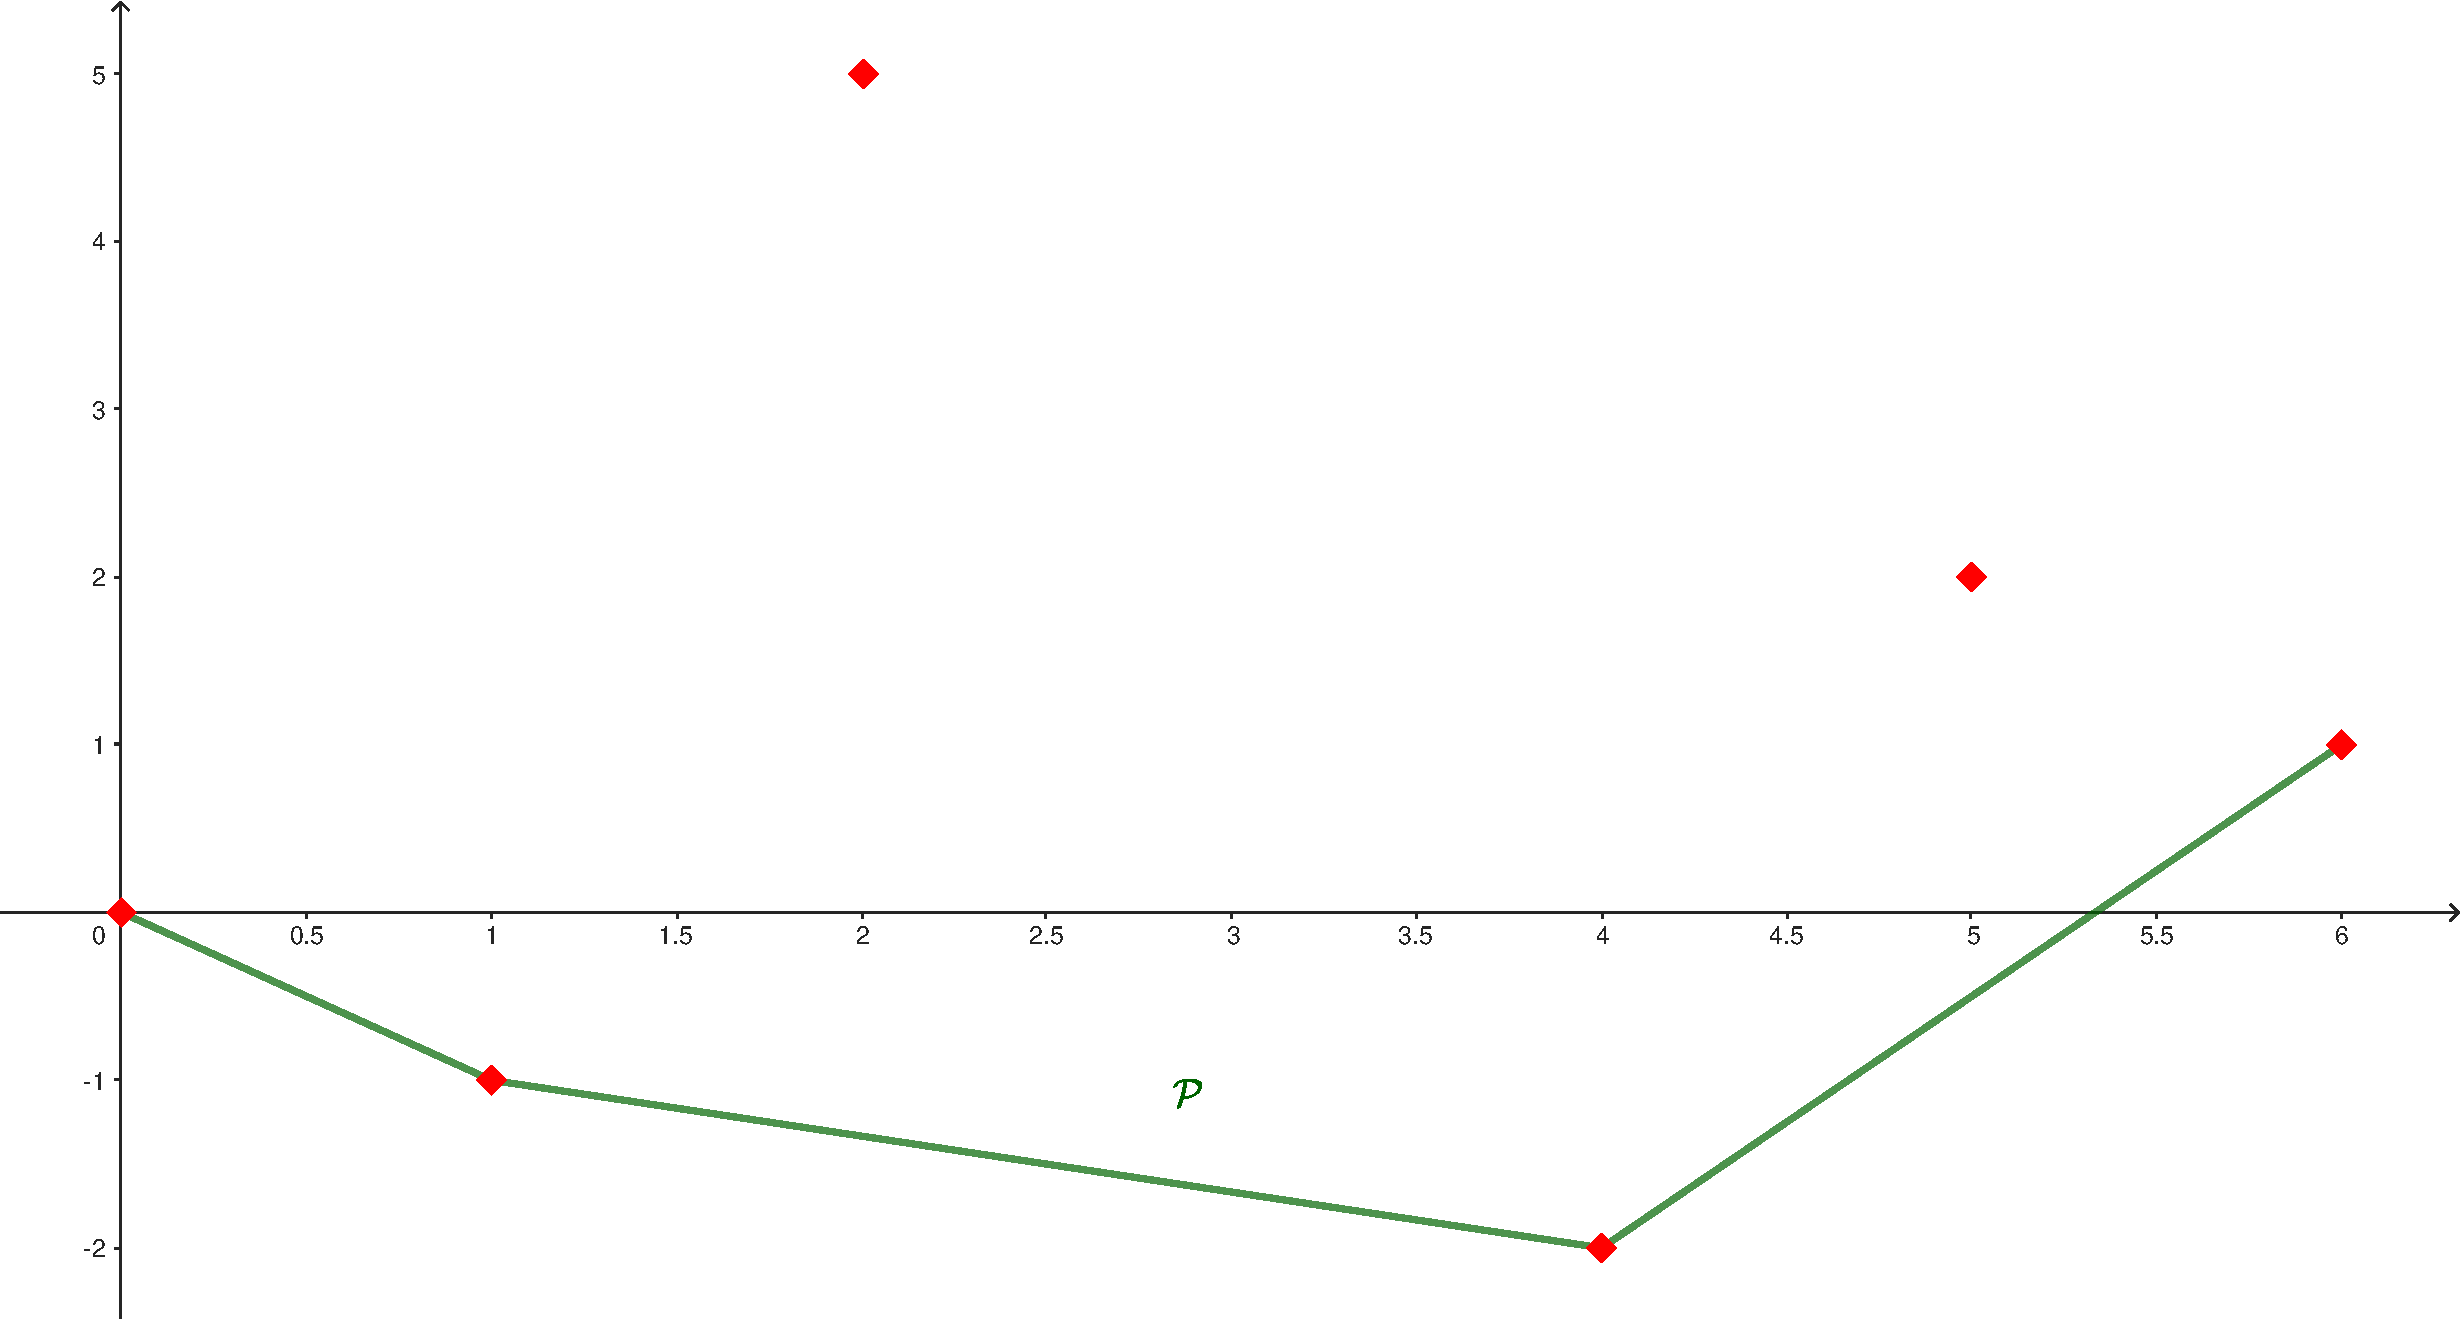
\includegraphics[scale=0.25]{figures/polygone_newton.pdf}
      \caption{Polygone de Newton $\mathcal{P}$ associé à $P$}
      \label{poly_newton}
    \end{figure}
  \end{ex}

On pourra alors prouver que l'enveloppe convexe inférieure ainsi définie est une ligne brisée constitués de segments de pentes deux à deux différentes. On appelle pentes du polygones les pentes des segments de la ligne brisée et longueur d'un segment de la ligne brisé la longueur du projeté du segment sur l'axe des abscisses. 

\begin{theoreme}
Les pentes du polygone de Newton $\mathcal{P}$ sont exactement les opposés des valuations des racines de $P$ (dans $\overline{\mathbb{Q}_{p}}$). De plus, le nombre de racines de valuation $v$ est égal à la longueur du segment de pente $-v$.
\end{theoreme}

On considère alors un polynôme $P =X^n \sum_{i=1}^{n-1} a_{i}X^i$ à coefficient dans $\mathbb{Q}_p$ unitaire. On remarque immédiatement que le point d'abscisse $n$ du polygone de Newton $\mathcal{P}$ associé à $P$ est d'ordonnée nulle. On en déduit alors que si un des coefficients $(a_{i})_{0\le i\le n-1}$ est de valuation strictement négative, $\mathcal{P}$ admet une pente strictement positive et donc $P$ admet une racine de valuation strictement négative. 

Par contraposée, on en déduit que si polynôme unitaire à coefficient dans $\mathbb{Q}_{p} $ est à racine positive alors il est élément de $\mathbb{Z}_p[X]$.
>>>>>>> afed46df6ee66c8447d25c77be41fc228335ae00

\end{proof} 
 
    \section{Forme normale de Smith}
\label{smith} 
On revient dans cette partie sur la construction de la forme normale de Smith d'une matrice ainsi que sur les principaux résultats sur cette dernière. Ces résultats sont utilisé dans l'algorithme présenté en section \ref{sectionalgo}.  Les preuves de cette section ont étés tirées de \cite{howard_rings_nodate}  puis rapportées au cas $p$-adique, là ou le cours original se place dans le cadre plus général des anneaux euclidiens.



\begin{rappel}
	On appelle forme normale de Smith d'une matrice $M \in \mathcal{M}_{m,n}\left(\mathbb{Q}_{p} \right) $ de rang $r$ l'unique matrice $S$ de la forme $$S =  
	\begin{pmatrix} p^{a_1} & \\
		 & \ddots \\
		 & & p^{ar}\\
		 & & & 0\\
		 & & & & \ddots \end{pmatrix} $$
		 telle que $a_1\le  \ldots\le a_r$ et $M =  Q^{-1} S P$ avec $P \in \mathcal{G}L_n\left( \mathbb{Z}_p \right) $ et $Q \in \mathcal{G}L_m\left( \mathbb{Z}_p \right) $.
\end{rappel}
\textbf{Remarque préliminaire} 
Soit $M$ une matrice de $\mathcal{M}_{m,n}\left(\mathbb{Q}_{p} \right) $. Pour $k \in \mathbb{N}$ suffisamment grand $M_k := p^k M$ est à coefficient dans$\mathcal{M}_{n}\left(\mathbb{Z}_p\right)$. Il suffit donc de montrer l'existence et l'unicité de la forme normale de Smith sur les matrices de $\mathcal{M}_{n}\left(\mathbb{Z}_p\right) $ pour l'avoir sur toutes les matrices à coefficients dans $\mathbb{Q}_{p}$.

\begin{proof} Existence de la forme normale de Smith.

On démontrera le résultat par récurrence sur $m+n$. 

Les résultats dans les cas $n+m= 0,1$ et $2$ étant immédiats, on a l'initialisation.

Soit $k \in \mathbb{N}$ tel que tout matrice $M \in M_{m,n}\left( \mathbb{Z}_{p}  \right) $ avec $m+n \le  k$ admettent une forme normale de Smith.

	Soient $m,n \in \mathbb{N}$ tels que $m+n = k+1$ et $M \in \mathcal{M}_{m,n}\left(\mathbb{Z}_p\right) $.

	Si $M$ est nulle le résultat est immédiat. On supposera donc $M \neq 0$. 
	On peut alors trouver un coefficient $\alpha$ de $M$ de valuation minimale $a_1$. En multipliant $M$ à droite et à gauche par des matrices de permutation on peut faire remonter ce coefficient en position $(1,1)$. $M$ est alors équivalente à une matrice $N$ de la forme :

	\[
N = 		\begin{pmatrix} \alpha & N_{1,2} & \ldots & N_{1,n} \\
			N_{2,1} & * & \ldots & *\\
			\vdots & \vdots & \ddots & \vdots \\
			N_{m,1} &* & \ldots & *\\
		\end{pmatrix} 
	.\] 
	On considère alors $\tilde{\alpha} := \alpha^{-1} p^{a_1}$ ainsi $\alpha\tilde{\alpha} = p^{a_1} $ et $\tilde{\alpha} \in \mathbb{Z}_p^\times $ conformément à \ref{lemmeinversible}.
Multiplier à gauche $N$ par la matrice $\text{diag}( \tilde{\alpha}, 0, \ldots,0)$ conserve l'équivalence dans $\mathbb{Z}_p$ \footnote{car on multiplie par une matrice de déterminant inversible dans $\mathbb{Z}_p$ et donc elle même inversible.} et permet d'obtenir une matrice $\tilde{N}$ :
	\[
\tilde{N} = 		\begin{pmatrix} p^{a_1} & \tilde{N}_{1,2} & \ldots & \tilde{N}_{1,n} \\
			N_{2,1} & * & \ldots & *\\
			\vdots & \vdots & \ddots & \vdots \\
			N_{m,1} &* & \ldots & *\\
		\end{pmatrix} 
	.\] 
	

On remarque en particulier que le passage de $N$ à $\tilde{N}$ ne modifie pas la valuation de ses éléments. Or $N$ s'écrivant comme permutation des coefficients de $M$ $p^{a_1} $ reste un coefficient de $\tilde{N}$ de valuation minimale. À ce titre pour tout $2\le i\le m$ il existe $q_{i} \in \mathbb{Z}_p$ tel que $\tilde{N}_{i,1} = p^{a_1}q_{i}$ et de même pour tout $2\le j\le n$ on dispose de $p_{j} \in \mathbb{Z}_p$ vérifiant $N_{1,j} = p^{a_1} p_{j}$. On fixe de tels $q_{i}$ et $p_{j}$. En ajoutant à la $i$-ième ligne de $\tilde{N}$ $q_{i}$ fois la première pour $2\le i\le m$ on annule alors tous les coefficients de la première ligne sauf $p^{a_1}$ en conservant l'équivalence.

	\[
 		\begin{pmatrix} p^{a_1}  & \tilde{N}_{1,2}- p^{a_1}  q_{i} & \ldots & \tilde{N}_{1,n}- p^{a_1}  q_{i} \\
			N_{2,1} & * & \ldots & *\\
			\vdots & \vdots & \ddots & \vdots \\
			N_{m,1} &* & \ldots & *\\
		\end{pmatrix} 
 = 		\begin{pmatrix} p^{a_1}& 0 & \ldots & 0 \\
			N_{2,1} & * & \ldots & *\\
			\vdots & \vdots & \ddots & \vdots \\
			N_{m,1} &* & \ldots & *\\
		\end{pmatrix} 
	.\] 

On procède alors pareillement pour les colonnes en ajoutant à la $j$-ième colonne de la matrice nouvellement obtenue $p_{j}$ fois la première pour obtenir une matrice dont le seul coefficient non nul de la première ligne et colonne est $p^{a_1}$.

	\[ 		\begin{pmatrix}  p^{a_1}& 0 & \ldots & 0 \\
			0 & * & \ldots & *\\
			\vdots & \vdots & \ddots & \vdots \\
			0 &* & \ldots & *\\
		\end{pmatrix} 
	.\] 

Dans les cas particuliers ou $m = 1$ ou $n=1$ la preuve s'arrête ici, la matrice étant de la forme demandée. 
Sinon les coefficients de la matrice nouvellement obtenue s'écrive comme sommes et produits de coefficients de $M$ et sont de valuation supérieure à $a_1$. On applique alors l'hypothèse de récurrence et obtient le résultat.
	\end{proof}

	\begin{remarques}
		On observe que la preuve ci-dessus décrit en fait une procédure permettant de canuler la forme normale de Smith d'une matrice ainsi que des matrices de passages associées en $O\left( \max\left( m,n \right) ^3 \right) $ opérations. Il est cependant possible d'obtenir ce même résultats en $\Omega( \max(m,n)) $, résultat prouvé par Tristan Vaccon et son stagiaire dans un article encore non publié.
	\end{remarques}



	\begin{proof} Unicité de la forme normale de Smith
		Soit $M \in \mathcal{M}_{m,n}\left(\mathbb{Z}_p\right) $ et $S = \begin{pmatrix} p^{a_1} & \\
		 & \ddots \\
		 & & p^{ar}\\
		 & & & 0\\
		 & & & & \ddots \end{pmatrix} $ sa forme normale de Smith.

		La preuve de l'unicité repose sur le fait que la valuation minimale pour les sous-déterminants de taille $k\times k$ de $M$ soit $a_1 + a_2 + \ldots + a_r$ si $k\le r$ et $0$ sinon pour $k=1,\ldots, \min(m,n)$. Ce qui permet de conclure immédiatement à l'unicité de $S$.

		On note pour toute matrice $A \in \mathcal{M}_{m,n}\left(\mathbb{Z}_{p} \right) $, $v_k(A)$ la valuation minimale des déterminants de taille $k\times k$ de A, pour $k=1\ldots \min\left( m,n \right) $.

		Remarquons tout d'abord la propriété suivante : pour tous $A \in \mathcal{M}_{m,n}\left(\mathbb{Z}_p\right) $ et $Q \in \mathcal{M}_{n}\left(\mathbb{Z}_p\right), v_k(AQ) \le v_k(A)$

	Le résultat est une conséquence immédiate de \ref{propval}.

	On en déduit alors ce résultat plus fort :
	Pour toutes matrice $A \in \mathcal{M}_{m,n}\left(\mathbb{Z}_p\right) $, $P \in \mathcal{G}L_n\left( \mathbb{Z}_p \right) $ et $Q \in \mathcal{G}L_m\left( \mathbb{Z}_p \right) $ on a $v_k(A) = v_k(PAQ)$. 

	En effet, soient $A\in \mathcal{M}_{m,n}\left(\mathbb{Z}_p\right) $, $P \in \mathcal{M}_{n}\left(\mathbb{Z}_p\right) $ et $Q \in \mathcal{M}_{m}\left(\mathbb{Z}_p\right) $.
	On a l'inégalité suivante par invariance de $v_k$ par transposition :
	$$v_k(PAQ) \le v_k(PA) = v_k\left( (PA)^T \right) = v_k(A^T P^T) \le v_k(A).$$
	Puis de même $v_k(A) = v_k(P^{-1}(PAQ)Q^{-1}) \le v_k(PAQ)$.


En appliquant ce résultat à $M$ et $S$ on a que pour tout $1\le k\le \max(m,n) $ $v_k(M)  = v_k(S)$, or par définition de $S$, $v_k(S) = a_1 + a_2 + \ldots + a_r$ si $k\le r$ et $0$ sinon. D'où le résultat.

	\end{proof}
     
    \section{Résolution de la programmation linéaire \texorpdfstring{$p$}{p}-adique} 
\label{appendixalgo} 
Cette section présente le pseudo-code ainsi qu'une implémentation en \sage de l'algorithme de la section \ref{sectionalgo}.
\renewcommand{\algorithmicrequire}{\textbf{Entrée:}}
\algrenewcommand{\algorithmicensure}{\textbf{Sortie:}}
%\algrenewcommand{\algorithmiccomment}[1]{\{#1\}}
\renewcommand{\algorithmicend}{\textbf{fin}}
\renewcommand{\algorithmicif}{\textbf{si}}
\algrenewcommand{\algorithmicthen}{\textbf{alors}}
\algrenewcommand{\algorithmicelse}{\textbf{sinon}}
\newcommand{\algorithmicelsif}{\algorithmicelse\ \algorithmicif}
\newcommand{\algorithmicendif}{\algorithmicend\ \algorithmicif}
\algrenewcommand{\algorithmicfor}{\textbf{pour}}
\algrenewcommand{\algorithmicforall}{\textbf{for tout}}
\algrenewcommand{\algorithmicdo}{\textbf{}}
\newcommand{\algorithmicendfor}{\algorithmicend\ \algorithmicfor}
\algrenewcommand{\algorithmicwhile}{\textbf{tant que}}
\newcommand{\Failwith}{\textbf{Échec : }}  

 

\begin{algorithm}
\caption{Résolution de la programmation $p$-adique}
%\Entry Une matrice $A$ de taille $m \times n$, un vecteur $b$ de taille $m$ et un vecteur $c$ de taille $n$.
\begin{algorithmic}[0]
\State $S,P,Q$ = FormeNormaleDeSmith($A$)
\State $r$ = rang($S$)
\State $b' = P \times b$
\State $c'$ = $c \times Q$
\For{$i$ allant de $r+1$ à $m$}
\If{$\val\left(b'[i] \right) < 0$}
\State Pas de solution
\EndIf
\EndFor
\For{$i$ allant de $r+1$ à $n$} 
\If{$c'[i]\neq 0$}
\State Le problème n'est pas borné
\EndIf
\EndFor
\State $\tilde{c} =$Projection$\left( c', 1, r \right) $ \Comment On réduit le problème à un problème de taille $r$ 
\State $\tilde{b} =$ Projection$\left(b', 1, r \right) $ 
\State $\tilde{S} = $SousMatrice$\left( S, (1,r),(1,r) \right) $
\State $\lambda_0 = \tilde{c}. S^{-1}. \tilde{b} $
\State $v_0 = \min \left\{\val\left(z_{i}\right)| \left( z_1,\ldots,z_r \right) = \tilde{c}.S^{-1}  \right\}$

\If{$\val\left( \lambda_0\right) < v_0$}
\Return $\val\left( \lambda_0 \right)$
\Else \Return $v_0$ \Comment Si l'on cherche à calculer la valuation maximale à la place il suffit de soulever une erreur au lieu de renvoyer $v_0$.
\EndIf
\end{algorithmic}
\end{algorithm}

Ou FormeNormaleDeSmith renvoie la forme normale de Smith de la matrice $A$ ainsi que les matrices $P$ et $Q$ telles que \todo{stick to a convention}. 

L'algorithme s'exécute en $O\left( n^3 \right) $
 

    \printbibliography
    
\end{document}
